\author{Philipp Dominik Bzdok}

\title{Bachelorarbeit Medientechnologie \linebreak \linebreak
Authentifizierungsverfahren für digitale Fernsignaturen auf Grundlage der Handy-Signatur}

\documentclass[11pt,a4paper,ngerman]{scrreprt}
\usepackage[T1]{fontenc}
\usepackage{fontspec}
\usepackage[ngerman]{babel}

\usepackage{fancyhdr}
\pagestyle{fancy}
\fancyhf{}
\setlength{\headheight}{14pt}
\fancyhead[R]{\textsl{\rightmark}}
\fancyfoot[R]{\thepage}

\fancypagestyle{plain}{%
    \renewcommand{\headrulewidth}{0pt}%
    \fancyhf{}%
    \fancyfoot[R]{\thepage}%
}
\addtokomafont{disposition}{\rmfamily}

\usepackage[style=alphabetic,backend=biber]{biblatex}
\addbibresource{Literaturverzeichnis.bib}

\usepackage{color}
\usepackage{tabularx}
\usepackage{booktabs}
\usepackage{amsmath}
\usepackage{amssymb}
\usepackage{graphicx}
\usepackage[skip=5pt,font=footnotesize]{caption}
\usepackage{csquotes}
\usepackage{enumitem}

\usepackage{todonotes}

\usepackage[titles]{tocloft}
\newlistof{listing}{lol}{Quellcodeverzeichnis}

\usepackage[newfloat]{minted}
\usemintedstyle{xcode}
\setminted[java]{linenos,tabsize=2,breaklines,fontsize=\footnotesize,frame=lines,framesep=2ex,autogobble}
\setminted[ruby]{linenos,tabsize=1,breaklines,fontsize=\footnotesize,frame=lines,framesep=2ex,autogobble}

\usepackage[bookmarksnumbered]{hyperref}
\hypersetup{pdfborder={0 0 0}, breaklinks=true}
\usepackage{bookmark}

\setlength{\parskip}{0.5em}
\setlength{\parindent}{0em}

\setlength{\cftlistingnumwidth}{3em}

\newcommand{\ruby}[1]{\mintinline{ruby}{#1}}

% !TEX root = Bachelorarbeit_Philipp_Bzdok

\begin{document}
\maketitle

% ----------------------------------------------------------------
% Preamble DE
% ---------------------------------------------------------------- 
\chapter*{Bachelorarbeit}
\textbf{Thema:}

Authentifizierungsverfahren für digitale Fernsignaturen auf Grundlage der Handy-Signatur
\\[4ex]
\textbf{Gutachter:}
\begin{enumerate}
    \item Prof. Dr.-Ing. Luigi Lo Iacono (Technische Hochschule Köln)
    \item Dipl.-Ing. Tobias Wagner (n-design GmbH)
\end{enumerate}
\textbf{Zusammenfassung:}

Die digitale Signatur stellt ein wichtiges Werkzeug der modernen Informationstechnik dar und durch Fernsignaturen ist es heutzutage möglich, digital, rechtsgültige Unterschriften zu leisten. Der Prozess der Signatur setzt dementsprechend eine starke Authentifizierung des Benutzers voraus. In diesem Kontext wird die SMS-TAN, das erste Authentifizierungsverfahren der österreichischen Handy-Signatur und das am weitesten verbreitete Zwei-Faktor Authentifizierungsverfahren, analysiert. Darauf aufbauend werden alternative Authentifizierungsverfahren für den Anwendungsbereich Fernsignatur evaluiert. Durch die prototypische Implementierung der TOTP und U2F Authentifizierungsverfahren wird gezeigt, wie mit überschaubarem Aufwand die unsichere SMS-TAN substituiert werden kann um somit ein höheres Sicherheitsniveau zu erreichen.
\\[4ex]
\textbf{Stichwörter:}

Authentifizierung, digitale Signatur, Kryptographieverfahren, SMS-TAN, TOTP, U2F
\\[4ex]
\textbf{Datum:}

\today
\clearpage

% ----------------------------------------------------------------
% Preamble EN
% ---------------------------------------------------------------- 
\chapter*{Bachelors Thesis}
\textbf{Title:}

Authentication procedures for digital remote signatures based on mobile phone signatures
\\[4ex]
\textbf{Reviewers:}
\begin{enumerate}
    \item Prof. Dr.-Ing. Luigi Lo Iacono (Technische Hochschule Köln)
    \item Dipl.-Ing. Tobias Wagner (n-design GmbH)
\end{enumerate}
\textbf{Abstract:}

The digital signature is an important tool of modern information technology and with remote signatures it is now possible to provide digital, legally valid signatures. Accordingly, the signature process requires a strong authentication of the user. In this context, the SMS-TAN, the first authentication procedure of the Austrian mobile phone signature and the most widespread two-factor authentication procedure, is analyzed. Based on this, alternative authentication methods for the field of remote signatures will be evaluated. Through the prototypical implementation of the TOTP and U2F authentication methods, it will be shown how the unsecure SMS-TAN can be substituted with a manageable effort in order to achieve a higher level of security.
\\[4ex]
\textbf{Keywords:}

Authentication, digital signature, cryptographic methods, SMS-TAN, TOTP, U2F
\\[4ex]
\textbf{Date:}

\today
\clearpage

% ----------------------------------------------------------------
% Eidesstattliche Erklärung
% ---------------------------------------------------------------- 
\chapter*{Eidesstattliche Erklärung}
Ich erkläre an Eides statt, dass ich die vorgelegte Abschlussarbeit selbständig und ohne fremde Hilfe verfasst, andere als die angegebenen Quellen und Hilfsmittel nicht benutzt und die den benutzten Quellen wörtlich oder inhaltlich entnommenen Stellen als solche kenntlich gemacht habe.

\vspace{1.5cm}

\_\_\_\_\_\_\_\_\_\_\_\_\_\_\_\_\_\_\_\_\_\_ \\
(Ort, Datum)

\vspace{0.5cm}

\_\_\_\_\_\_\_\_\_\_\_\_\_\_\_\_\_\_\_\_\_\_ \\
(Unterschrift)

\clearpage

% ----------------------------------------------------------------
% Vorwort
% ---------------------------------------------------------------- 
\chapter*{Vorwort}
Hier möchte ich auf die Umstände der Abschlussarbeit eingehen und denen danken, die mir dabei geholfen haben.
\clearpage

% ----------------------------------------------------------------
% Inhaltsverzeichnis
% ---------------------------------------------------------------- 
\tableofcontents
\clearpage

% ----------------------------------------------------------------
% Inhalt
% ----------------------------------------------------------------

\chapter{Einleitung}
Digitale Signaturen nehmen in der heutigen Zeit eine wichtige Rolle in der Informationstechnik und somit im Alltag ein. Mit Hilfe von digitalen Signaturen ist es möglich beliebigen digitalen Daten zweifelsfrei Integrität, Authentizität und nicht-Abstreitbarkeit nachzuweisen. Die Eigenschaften der Integrität, Authentizität und nicht-Abstreitbarkeit sind besonders wichtig im juristischen Kontext der elektronischen Signatur, in welchem sie das Gegenstück zur handschriftlichen Unterschrift bildet. Der Begriff \emph{elektronische Signatur} wird oft synonym zur \emph{digitalen Signatur} verwendet, jedoch ist die elektronische Signatur ein juristischer Begriff, welcher erstmals in einem überarbeiteten Entwurf der EU-Richtlinie 1999/93/EG von der EU-Kommission verwendet wurde \cite{eSigEU99}. Der Begriff digitale Signatur hingegen stammt aus der Mathematik beziehungsweise aus der Kryptographie und bezeichnet einerseits ein asymmetrisches Kryptographieverfahren, und anderseits den mathematischen Wert, welcher durch das Kryptographieverfahren erzeugt wird.

Digitale Signaturen werden bereits in einem breiten Spektrum von Anwendungen eingesetzt, wie zum Beispiel für Schutz von E-Mail oder Zertifikatsbasierten Systemen. Des weiteren werden digitale Signaturen immer häufiger in neuen Anwendungsbereichen eingesetzt. Eine besondere Anwendung auf die ich im Laufe dieser Ausarbeitung explizit eingehen möchte, ist die österreichische \textit{Handy-Signatur}. Die \textit{Handy-Signatur} ermöglicht es den Bürgern Österreichs sich ohne zusätzliche Hardware wie Kartenlesegeräte online per Handy auszuweisen oder Formulare und Dokumente elektronisch zu unterschreiben \cite{handySigOnline}. Die Besonderheit dieser digitalen Signatur ist, dass die \textit{Handy-Signatur} eine qualifizierte elektronische Signatur auslöst und somit juristisch einer handgeschriebenen Unterschrift gleichgesetzt werden kann. Deshalb erfordert eine solche elektronische Signatur eine \emph{starke} Benutzer-Authentifizierung, welche in der Praxis durch eine Kombination von Passwort und \textit{SMS-TAN} oder andere Authentifizierungsverfahren implementiert wird. Die \textit{SMS-TAN} wurde jedoch bereits von NIST\footnote{National Institute of Standards and Technology} in ihrer Tauglichkeit eingeschränkt, da SMS nie dafür gemacht worden ist Geheimnisse zu übertragen \cite{mobileSec,NIST800-63B}. Trotz der mangelhaften Eignung von SMS als Kanal für Out-Of-Band Authentifizierung\footnote{Authentifizierung über separaten Kanal}, ist das SMS-OTP\footnote{One time password} die am meisten verbreitete Variante der Multi-Faktor Authentifizierung \cite[Abb. 3]{fido17}.

Aus diesem Grund möchte ich in dieser Arbeit die Eigenschaften der Authentifizierungsverfahren der \textit{Handy-Signatur} beleuchten und darauf basierend Alternativen evaluieren und prototypisch implementieren. Mein Ziel ist es, die modernen Möglichkeiten von Multi-Faktor Authentifizierung im Kontext der elektronischen Signatur zu vergleichen und zu bewerten, um abschließend eine Aussage über die Tauglichkeit für den Anwendungsbereich \textit{Fernsignatur} machen zu können.

\section*{Abgrenzung}
Die digitale (Fern-)Signatur besteht aus vielen komplexen Verfahren, wie Hashfunktionen, Kryptographieverfahren, Smartcards, uvm.. Diese möchte ich nur der Vollständigkeit halber erläutern. In diesen Bereichen werde ich mich nur auf bereits veröffentlichte Methodiken stützen und von ihnen Gebrauch machen. Insbesondere setze ich bestimmte Rahmenbedingungen für die Implementierungen der Prototypen voraus, wie gesicherte Übertragunskanäle, sichere Schlüsselerzeugung, sichere Schlüsselspeicherung, sichere Zufallsgeneratoren und sichere Signaturerstellungseinheiten, da diese außerhalb der eigentlichen Authentifizierung fungieren.
\clearpage


\chapter{Grundlagen}
Um die Eignung von Authentifizierungsverfahren bestimmen zu können, müssen erst einmal die Rahmenbedingung festgelegt werden. Die digitale Signatur und die \textit{Handy-Signatur} werden im Folgenden beleuchtet, da dies der Anwendungsbereich ist, welchen die Authentifizierungsverfahren schützen sollen. Dazu stelle ich verschiedenste Signaturvarianten und deren Komponenten im Detail dar. Nach der Bestimmung dieser Eigenschaften wird die Authentifizierung im Kontext der Signatur erläutert.

\section{Kryptographische Verfahren}
\subsection{Hash-Funktionen}\label{sec:Hash-Funktionen}
\textit{Hash-Funktionen} spielen eine zentrale Rolle in der Welt der Kryptographie und \textit{digitalen Signaturen}. Allgemein bilden diese Funktionen eine Nachricht beliebiger (Bit-)Länge auf einen Hash-Wert festen Länge ab. Der Hash-Wert ist abhängig von der gesamten Nachricht und sollte möglichst schnell berechnet werden können. Dietmar Wätjen beschreibt die Kollisionsfreiheit als eine besondere Eigenschaft von \textit{Hash-Funktionen} \cite[S. 89]{krypt08}: 
\begin{quote}
    ``Es sei $M$ eine Nachricht. Eine Hashfunktion $h$ ist \emph{schwach kollisionsfrei für $M$} [...], wenn es berechnungsmäßig praktisch unmöglich ist, eine Nachricht $M' \neq M$ mit $h(M) = h(M')$ zu finden. [...]
    Eine Hashfunktion ist \emph{stark kollisionsfrei} [...], wenn es berechnungsmäßig praktisch unmöglich ist, Nachrichten $M$ und $M'$ mit $M' \neq M$ und $h(M') = h(M)$ zu finden.''
\end{quote}
Für die Verwendung von \emph{Hash-Funktionen} im Kontext der Signatur muss die Funktion eine sogenannte \emph{Einweg-Hash-Funktion} sein, wie in \cite[S. 99]{krypt08} beschrieben:
\begin{quote}
    ``Eine Hashfunktion ist eine \emph{Ein-Weg-Funktion} [...], wenn es für einen gegebenen Fingerabdruck $z$ berechnungsmäßig praktisch unmöglich ist, eine Nachricht $M$ mit $h(M)=z$ zu finden.''
\end{quote}
Implizit ergibt sich aus der Forderung nach stark kollisionsfreien \textit{Hash-Funktionen} auch die Eigenschaften der Ein-Weg-Funktionen \cite[S. 99]{krypt08}.

Die \textit{Hash-Funktionen} sind so wichtig für die \textit{digitalen Signaturen}, da bei den gängigen Signaturvarianten nur der Hash-Wert der Nachricht signiert wird und nicht die Nachricht selbst. Wichtige Funktionen in diesem Kontext, die in ihrer Sicherheit stetig durch führende Institutionen (NIST\footnote{National Institute of Standards and Technology - Secure Hash Standard \cite{shs180-4}}, SOG-IS\footnote{Senior Officials Group Information Systems Security \cite{sogisACM}}/BSI\footnote{Bundesamt für Sicherheit in der Informationstechnik \cite{bsi-tr-02102-1}}, etc.) geprüft werden, sind:
\begin{table}[h]
    \begin{tabularx}{\textwidth}{ lX }
        \toprule
        Familie & Ausprägungen \\ 
        \midrule
        SHA2 & SHA-256, SHA-512/256, SHA-384 und SHA-512 \\
        SHA3 & SHA3-256, SHA3-384, SHA3-512 \\
        \bottomrule
    \end{tabularx}
    \caption{Empfohlene Hash-Funktionen}
    \label{table:Hashfunktionen}
\end{table}

Eine Signatur soll die Eigenschaften Integrität und Authentizität der zu signierenden Daten sicherstellen. Damit die Authentizität gewährleistet werden kann, muss erst die Integrität der Nachricht sicher gestellt werden. An dieser Stelle greifen die Eigenschaften der \textit{Hash-Funktion}. Dadurch, dass nur der Hash-Wert signiert wird, kann der Empfänger der Signatur durch eine eigene Hash-Wert Berechnung der Nachricht nachvollziehen, dass die Nachricht nicht verändert worden ist\footnote{Durch die Änderung der Nachricht würde auch die Signatur ungültig werden}. Außerdem bietet die Signatur des Hash-Wertes mit fixer Länge Laufzeitvorteile in einigen Signaturverfahren.

\subsection{Digitale Signaturen}\label{sec:signatur}
Als \textit{digitale Signatur} bezeichnet man im allgemeinen ein asymmetrisches Kryptosystem\footnote{Oberbegriff für Public-Key-Verschlüsselungsverfahren}. Bei asymmetrischen Kryptographiesystemen besitzt jeder Teilnehmer ein Schlüsselpaar, bestehend aus einem \emph{öffentlichen Schlüssel} und einem \emph{privaten Schüssel}. Der \emph{private Schlüssel} wird für die Signaturerstellung verwendet, wobei der \emph{öffentliche Schlüssel} von einer beliebigen anderen Person abgerufen werden kann, um die Signatur zu verifizieren (siehe Abb. \ref{fig:Signaturablauf}). Da ausschließlich der Teilnehmer selbst Zugang zu seinem eigenen \emph{privaten Schlüssel} hat, eignet sich ein solches System hervorragend zur Sicherstellung von Authentizität von Daten und somit für die \textit{digitalen Signatur}. Authentizität ist eine der fünf wichtigen Eigenschaften einer Signatur \cite{sch05}:
\begin{enumerate}
    \item Sie ist \textbf{authentisch}. Das bedeutet, dass der Unterzeichner die Signatur willentlich ausgeführt hat.
    \item Sie ist \textbf{fälschungssicher}. Das bedeutet, dass die Signatur ausschließlich vom Unterzeichner ausgeführt worden ist und von niemand anderen.
    \item Sie ist \textbf{nicht wiederverwertbar}. Das bedeutet, dass die Signatur nur auf einer Nachricht gültig ist.
    \item Die signierte Nachricht ist \textbf{unveränderbar}. Das bedeutet, dass die Nachricht nach der Signatur nicht modifiziert werden kann.
    \item Die Signatur ist \textbf{bindend}. Das bedeutet, das der Unterzeichner diese zu einem späteren Zeitpunkt nicht annullieren oder bestreiten kann. Diese Eigenschaft ist das Ergebnis der Summe der Eigenschaften 1-4 und ist besonders im juristischen Kontext der elektronischen Signatur relevant.
\end{enumerate}
\begin{figure}[h]
    \centering
        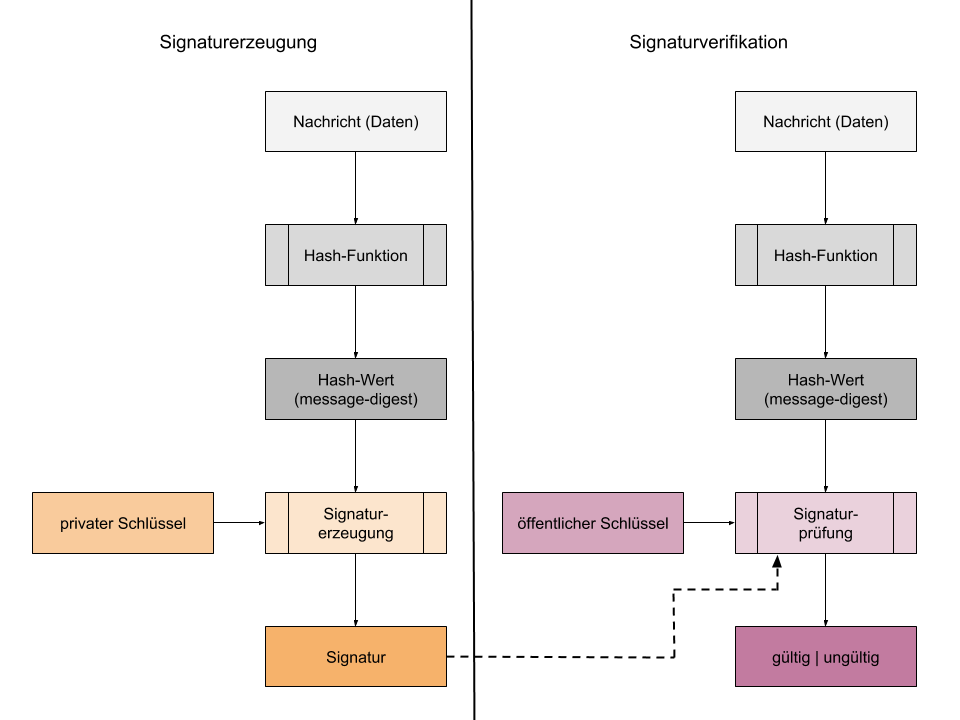
\includegraphics[width=\textwidth]{Abbildungen/Ablauf_Signatur.png}
    \caption{Schematischer Ablauf der Signaturerzeugung und Verifikation}
    \label{fig:Signaturablauf}
\end{figure}

Es gibt Grundsätzlich zwei Arten eine Nachricht $M$ digital zu signieren, wobei $S$ und $V$ zwei Personen sind \cite[S. 28-29]{kryptSec11}:
\begin{enumerate}
    \item Signatur mit Nachrichten-Rückgewinnung: Die Nachricht $M$ wird ohne Vorverarbeitung mit dem \emph{privaten Schlüssel} $d_s$ von $S$ signiert, sodass die daraus resultierende Signatur die Form $s = f_{d_s}(M)$ hat. Diese Nachricht kann von $V$ wiederum durch den \emph{öffentlichen Schlüssel} $e_s$ von $S$ dechiffriert und die ursprüngliche Nachricht wiederhergestellt werden: $M = f_{e_s}(f_{d_s}(M))$. Nur geeignet für Nachrichten kürzer als die Schlüssellänge. Diese Variante der Signatur wird im ISO/IEC-Standard 9796-2 definiert.
    \item Signatur mit Hash-Wert Anhang: Die Nachricht $M$ wird mit Hilfe einer Hash-Funktion\footnote{Siehe Abschnitt \ref{sec:Hash-Funktionen}} $h(M)$ auf einen Wert mit konstanter Länge (z.B. 160 Bit) abgebildet. Die Signatur hat somit die Form $s = f_{d_s}(h(M))$ und wird zusätzlich zur Nachricht übertragen. Die Person $V$ kann nun den Hash-Wert der Nachricht $M$ durch $h(M) = f_{e_s}(f_{d_s}(h(M))$ errechnen. Auch geeignet für längere Nachrichten.
\end{enumerate}
In der Praxis findet größtenteils nur die Signatur mit Hash-Wert Anhang Verwendung, da sonst die Signatur linear mit der Größe der Nachricht wächst und eine längere Nachricht eine größere Angriffsfläche bietet. Welche Signaturalgorithmen $f_{d_s}(h(M))$ in der Praxis verwendet werden, wird hauptsächlich über den fortlaufend aktualisierten ``Digital Signature Standard (DSS)'' des National Institute of Standards and Technology in den USA vorgegeben. Dieses Dokument stellt Empfehlungen dar, welche Signaturalgorithmen als sicher angesehen werden können und wie diese zu verwenden sind. Auf europäischer Ebene veröffentlicht die SOG-IS Crypto Working Group das sogenannte ``SOG-IS Crypto Evaluation Scheme Agreed Cryptographic Mechanisms'' \cite{sogisACM}. Insbesondere die Verfahren \textit{RSA} und \textit{DSA} haben sich durchgesetzt und werden häufig eingesetzt, jedoch besteht eine Tendenz zu den Signaturverfahren auf Basis von elliptischen Kurven da diese Vorteile in der Sicherheit, der Schlüssellängen und der Laufzeit gegenüber \textit{RSA} und \textit{DSA} aufweisen \cite[S. 59]{komSec13}

Auf Grundlage der Empfehlung der SOG-IS möchte ich zur Übersicht die gängigen Signaturverfahren aufzählen:
\subsubsection{RSA}
Der \textbf{R}iverst-\textbf{S}hamir-\textbf{A}dleman Algorithmus ist ein Public-Key Kryptosystem und findet oft Anwendung in Bereichen der Verschlüsselungsverfahren. Jedoch kann dieser Algorithmus auch zur Signatur von Nachrichten eingesetzt werden. 
\begin{quote}
    ``Die Sicherheit von RSA basiert auf der Schwierigkeit, große Zahlen in ihre Primfaktoren zu zerlegen.'' \cite[S. 82]{ertel12}
\end{quote}
\begin{description}[font=\rmfamily]
    \item[Schlüsselerzeugung:] Zwei stochastisch unabhängige Primzahlen $p$ und $q$ werden generiert, wobei $p \neq q$. Die beiden Primzahlen sollten so groß gewählt werde, dass das RSA-Modul $n=p \cdot q$ die gewünschte Stellenlänge hat. Das Schlüsselpaar besteht aus $e$ (encrypt) und $d$ (decrypt) und wird mit Hilfe der Eulerschen Funktion ermittelt:
    \[
        \Phi(n = p \cdot q) = (p-1) \cdot (q-1)
    \]
    Einer der beiden Schlüssel wird zufallsmäßig gewählt, sodass er kleiner ist als $\Phi(n)$ und teilerfremd zu $\Phi(n)$ ist. Der andere Schlüssel ergibt sich aus der Bedingung für RSA, dass die beiden Schlüssel $e$ und $d$ eines Paares multiplikativ invers in der Arithmetik modulo $\Phi(n)$ sind:
    \[
        e \cdot d \equiv 1 (\bmod \Phi(n)) 
    \]
    Der \emph{private Schlüssel} $d$ ist geheim und muss durch spezielle Maßnahmen geschützt werden, da er für die Signatur benutzt wird. Der \emph{öffentliche Schlüssel} $e$ und der Modulo $n$ werden veröffentlicht und dienen zur Verifikation der Signatur. Die Primzahlen $p$ und $q$ müssen ebenfalls sicher verwahrt werden. Sie können aber auch vernichtet werden um Missbrauch vorzubeugen.
    \item[Signaturerzeugung:] Voraussetzung für die Signaturerzeugung, ist die Formatierung\footnote{RSA-Padding} des Hash-Wertes auf die Länge des Moduls $n$. Die Signatur $s$ für die Nachricht $M$ kann nun berechnet werden durch:
    \[
        s = (M^d) \bmod n    
    \]
    \item[Signaturverifikation:] Die Signatur kann wiederrum unter Kenntnis des \emph{öffentlichen Schlüssels} bestehend aus $(e, n)$ verifiziert werden:
    \[
        (s^e) \bmod n = (M^d)^e \bmod n = M'
    \]
    Falls die wiederhergestellte Nachricht $M'$ mit der übertragenen Nachricht $M$ übereinstimmt, so kann die Signatur als gültig angesehen werden.
    \item[Anmerkungen:] Bei RSA handelt es sich um ein deterministisches Verfahren. In der Praxis wird statt der unmittelbaren Nachricht der Hash-Wert dieser Nachricht signiert. In diesem Fall muss $m$ mit $h(m)$ ersetzt werden. Besonders die Erzeugung der Zufallszahlen und der \emph{private Schlüssel} sind von besonderer Wichtigkeit und müssen durch spezielle Verfahren geschützt werden, auf die ich in Kapitel \ref{sec:Authentifizierung} noch detailliert eingehen werde.
\end{description}
\subsubsection{Digital Signature Algorithm (DSA)}
Dieses Signaturverfahren wurde erstmals 1991 vom National Institute of Standards and Technology vorgeschlagen und letztendlich auch im Jahr 1994 als Standard im Digital Signature Standard (DSS) offiziell aufgenommen.
\begin{quote}
    ``Die Sicherheit dieses Verfahrens beruht auf der [..] Schwierigkeit des Diskreten Logarithmenproblems $\mathbb{F}^*_p$.'' \cite[S. 45]{bsi-tr-02102-1}
\end{quote}
Im Gegensatz zu RSA eignet sich dieses Verfahren nicht zur kryptographischen Verschlüsselung von Nachrichten, sondern ist speziell für den Anwendungsbereich der \textit{digitalen Signaturen} eingeführt worden. Ein weiterer Unterschied zu RSA ist die Notwendigkeit einer kryptographischen Hash-Funktion zur Signaturerzeugung.
\begin{description}[font=\rmfamily]
    \item[Schlüsselerzeugung:] Wähle zwei Zahlen, welche durch den Standard definiert sind und die Sicherheit des Verfahrens vorgeben:
    \[
        (L, N) \in \{(1024, 160), (2028, 224), (2048, 256), (3072, 256)\}
    \]
    Anschließend werden die Primzahlen $p$ und $q$ mit folgenden Eigenschaften erzeugt:
    \[
        2^{N-1} < q < 2^N \quad\textrm{,}\quad 2^{L-1} < p < 2^L \quad\textrm{und}\quad q|(p-1)
    \]
    Zusätzlich wird eine Zahl $\alpha \in \mathbb{F}^*_p$ gewählt und $g$ berechnet:
    \[
        g := \alpha^{(p-1)/q} \bmod p
    \]
    Falls $g = 1$ wiederhole die Berechnung von $g$ mit einem anderen $\alpha \in \mathbb{F}^*_p$. Der letzte Schritt der Schlüsselerzeugung besteht aus der Wahl einer Zahl $x \in \{1, \ldots, q - 1 \}$ und $y := g^x \bmod p$. Der \emph{öffentliche Schlüssel} setzt sich zusammen aus $(p, q, g, y)$ und der \emph{private Schlüssel} aus $x$.
    
    Wie auch bei RSA, wird der \emph{private Schlüssel} zur Signaturerzeugung genutzt und muss geschützt werden. Der \emph{öffentliche Schlüssel} dient wiederum auch der Verifikation der Signatur.
    \item[Signaturerzeugung:] Die Erzeugung der Signatur benötigt eine Hash-Funktion. Dabei sollte eine empfohlene Funktion aus der Tabelle \ref{table:Hashfunktionen} verwendet werden. Der aus der Funktion resultierende Hash-Wert sollte der Bit-Länge von $q$ entsprechen. Ebenso sollte die Länge von $p$ mindestens 2000 betragen\footnote{Bis 2022 als sicher eingestuft.\cite{bsi-tr-02102-1}}.

    Zur Berechnung wird noch eine Zufallszahl $k \in \{ 1, \ldots, q - 1 \}$ aus einem kryptographisch sicheren Zufallszahlengenerator benötigt. Diese Zahl wird pro Signatur erzeugt und muss, wie der \emph{private Schlüssel}, sicher verwaltet werden. Die Signatur einer Nachricht $M$ welche durch das DSA Verfahren generiert wird, besteht aus dem Zahlenpaar $r$ und $s$:
    \[
        r = (g^k \bmod p)
    \]
    Zur Berechnung von $s$ muss außerdem eine Zahl $z$ bestimmt werden aus den linkesten $N$ Bits des Hash-Wertes $h(M)$:
    \[
        s = (z + xr)k^{-1} \bmod q
    \]
    Die Signatur, bestehend aus $(s, r)$ kann nun zusammen mit der Nachricht $M$ verifiziert werden.
    \item[Signaturverifikation:] Um die Signatur, bestehend aus $(s, r)$, auf der Nachricht $M$ zu prüfen, bedarf es des \emph{öffentlichen Schlüssels} $(p, q, g, y)$ des Unterzeichners. Im ersten Schritt wird überprüft ob: 
    \[
        0 < r < q \quad\textrm{und}\quad 0 < s < q
    \]
    Falls einer dieser beiden Bedingungen nicht erfüllt werden, ist die Signatur als ungültig anzusehen. Damit die Signatur als gültig angesehen werden kann, muss $v$ berechnet werden durch:
    \begin{align*}
        v& = (((g)^{u1}(y)^{u2}) \bmod p) \bmod q \quad\textrm{, mit}\\
        w& = (s)^{-1} \bmod q \\
        z& = \textrm{linkeste N Bits von $h(M)$} \\
        u1& = (zw) \bmod q \\
        u2& = (rw) \bmod q
    \end{align*}
    Falls $v = r$, ist die Signatur gültig.
    \subsubsection{Anmerkungen}
    Im Gegensatz zur RSA-Signaturvariante handelt es sich hierbei um einen probabilistischen Algorithmus, da die zufällige Wahl des \emph{privaten Schlüssels} mit $x \in \{1, \ldots, q - 1 \}$ essenziell ist. Wichtige schützenswerte Merkmale dieses Verfahrens sind der \emph{öffentliche Schlüssel} $x$ und die Zufallszahl $k$ aus der Signaturerzeugung. Neben der hier dargestellten Variante des DSA Signaturalgorithmus über einen Galoiskörper, gibt es außerdem noch die Variante unter der Verwendung von Elliptischen Kurven (ECDSA).
\end{description}

\section{Authentifizierungsverfahren}\label{sec:Authentifizierung}
Als \emph{Authentifizierung} bezeichnet man den Nachweis einer behaupteten Eigenschaft einer Entität. Diese Entität kann beispielsweise eine Person oder ein Dokument sein. Das verwandte Wort \emph{Authentifikation} bezeichnet hingegen die Prüfung der Echtheit der Eigenschaft.
\begin{quote}
    ``Bei der Authentifikation gibt es zwei Rollen: Die eine Partei, die ihre Identität nachweisen will (Beweisende, ``prover'') und die andere Partei, die den Beweis nachprüft (Verifizierende, ``verifier''). Das Wort \emph{authentisieren} bezeichnet die beweisende Rolle und das Wort \emph{authentifizieren} bezeichnet die verifizierende Rolle. Mit dem Wort \emph{Authentifikation} werden beide Rollen zusammengefasst. Der Sprachgebrauch ist jedoch nicht ganz einheitlich.'' \cite[S. 149]{kryptSec11}
\end{quote}
\subsection{Verfahren}
Die Verfahren der Authentifizierung können in drei Kategorien eingeteilt werden:
\begin{description}[font=\rmfamily]
    \item[Wissen:] Eine Person kann sich durch das Wissen einer bestimmten Information gegenüber einer zweiten Partei authentisieren. Für die Authentifizierung durch Wissen sind in der Regel keine Hilfsmittel notwendig, da sie auf immateriellem Gut basiert. Jedoch hat dies auch Nachteile, wie z.\,B. dass Informationen vergessen, vervielfältigt oder erraten werden können. Beispiele für Authentifikation anhand von Wissen sind:
    \begin{itemize}
    \item Passwort
    \item PIN
    \item Sicherheitsfrage
    \end{itemize} 
    \item[Besitz:] Durch die Verwendung eines Besitztums kann sich eine Person gegenüber einer zweiten Partei authentisieren. Besitz ist immer etwas materielles und kann deshalb nicht einfach vervielfältigt werden. Der Besitzer muss jedoch die sichere Verwahrung sicherstellen, da der Gegenstand sonst verloren gehen oder sogar gestohlen werden könnte. Es liegt auch in der Verantwortung des Besitzers den Gegenstand, mit dem er sich authentisiert, nicht weiterzugeben. Beispiele von Authentifikation durch Besitz sind:
    \begin{itemize}
        \item Schlüssel
        \item USB Stick
        \item Smartcard
        \item Zertifikat
        \item Transaktionsnummer (TAN)
        \item Einmalpasswort (OTP)
    \end{itemize}
    \item[Körperliches Merkmal / Biometrie:] Durch Merkmale des Benutzers selbst kann dieser sich gegenüber einer zweiten Partei authentisieren. Biometrische Merkmale sind in der Regel öffentliche Informationen, wie Gesichts- oder Augenmerkmale, die der Benutzer immer mit sich trägt. Diese Eigenschaften können nicht weitergegeben werden, benötigen für die Erkennung jedoch in den meisten Fällen spezielle Technik. Außerdem kann die Erkennung nur mit einer Gewissen Wahrscheinlichkeit erfolgen, da sich die Merkmale im Laufe der Zeit verändern können. Beispiele von Authentifikation durch Biometrie sind:
    \begin{itemize}
        \item Fingerabdruck
        \item Gesichtserkennung
        \item Stimmerkennung
        \item Iriserkennung
        \item Handschrift
        \item Erbinformationen
        \item Tippverhalten
    \end{itemize}
\end{description}
Durch eine Kombination von den obigen Authentifizierungsverfahren entsteht eine sogenannte \emph{starke Authentisierung}. Ein gängiges Beispiel für eine Zwei-Faktor Authentifikation ist ein Geldautomat: Durch den Besitz der Chipkarte und das Wissen der PIN kann eine Authentifikation in zwei Stufen durchgeführt werden.

Die Authentifizierung im Kontext digitale Signaturen hat einen besonderen Stellenwert, da durch die Signatur rechtsverbindliche Verträge unterzeichnet werden können. Zum Schutz der kryptographischen Schlüssel, welche zur Signaturerstellung notwendig sind, wird die \emph{starke Authentisierung} implementiert. Dazu muss sich der Benutzer im Falle der Handy-Signatur, der A-Trust GmbH gegenüber mit Passwort (Wissen, erster Faktor) und einem zweiten Faktor (SMS-TAN, QR-OTP, SE) authentisieren.

\subsection{Vergleich}\label{sec:AuthentifizierungVergleich}
Die oben genannten Authentifizierungsverfahren werden im Folgenden in den Kategorien \emph{Benutzerfreundlichkeit}, \emph{Komplexität} und \emph{Sicherheit} im Kontext der serverseitigen mobilen Signatur verglichen. Die Kategorie Benutzerfreundlichkeit wurde gewählt, da in erster Linie der Benutzer eine Authentisierung durchführen muss. Die Kategorie Komplexität hingegen dient zur Analyse der technischen Umsetzungsmöglichkeiten. Im Anschluss wird die Sicherheit der Verfahren verglichen, wobei die Ergebnisse der Kategorien Benutzerfreundlichkeit und Komplexität eingehen werden.
\subsubsection{Benutzerfreundlichkeit}
Die Marktanalyse der FIDO Alliance \cite{fido17} zeigt eindeutig, dass die Authentifizierung durch Wissen (insbesondere Passwörter) deutlich verbreiteter ist als die übrigen Verfahren. Authentifizierung durch Passwörter und PIN sind heutzutage überall anzutreffen und nicht mehr wegzudenken. Diese Adaption zeigt eindeutig, dass sich dieses Authentifizierungsverfahren in Bezug Benutzerfreundlichkeit ebenfalls durchsetzen kann. Für dieses Verfahren braucht der Benutzer im idealfall keinerlei Hilfsmittel. Die Biometrische Authentifikation ist ebenfalls, aus Sicht des Benutzers, unkompliziert und erfordert keine Hilfsmittel. Lediglich das Gerät an welchem der Benutzer die Authentifizierung durchführen möchte muss die Technik dafür bereitstellen, z.\,B. der Fingerabdrucksensor des Smartphones. Stehen diese technischen Vorraussetzungen jedoch nicht zur Verfügung, muss der Benutzer eine Alternative wählen oder die entsprechende Hardware zur Verfügung stellen. Das wiederum verringert die Benutzerfreundlichkeit dieses Verfahrens. Grundsätzlich ist die Authentifizierung durch Besitz das Verfahren mit der geringsten Benutzerfreundlichkeit, da der Benutzer diesen für die Anwendung anschaffen und verwalten muss. 

Zusammenfassend werden die Eigenschaften der Authentifizierungsverfahren im Bezug zur Benutzerfreundlichkeit in Tabelle \ref{table:Benutzerfreundlichkeit} verglichen.
\begin{table}[htbp]
    \begin{tabularx}{\textwidth}{ lXX }
        \toprule
        Verfahren & Vorteile & Nachteile \\ 
        \midrule
        Wissen & Benutzer Benötigt keine Hilfsmittel & Kann vom Benutzer vergessen werden \\
         & immateriell & Eventuell schwierig sich viele Passwörter zu merken \\
        \midrule
        Besitz & Kann bekannter Gegenstand sein (z.\,B. Chipkarte) & Muss sicher verwahrt werden, da materiell \\
         & & Anschaffung (Kosten) \\
         & & Kann verloren gehen \\
         & & Kann gestohlen werden \\
        \midrule
        Biometrie & Merkmale trägt Benutzer immer bei sich & Merkmale sind öffentliche Informationen \\
         & & Gerät muss Funktionalität bereitstellen \\
        \bottomrule
    \end{tabularx}
    \caption{Vergleich der Benutzerfreundlichkeit von Authentifizierungsverfahren}
    \label{table:Benutzerfreundlichkeit}
\end{table}
\subsubsection{Komplexität}
Die Komplexität eines Authentifizierungsverfahrens hängt im Wesentlichen vom Maß der Sicherheit ab, welche diese bietet. Jedoch spielen auch andere Faktoren eine große Rolle, wie z.\,B. die Varianz der Eingangsparameter und die Verfügbarkeit von Hardware und Software. Ein Beispiel für ein Authentifizierungsverfahren mit geringer Komplexität ist die Passwortauthentifizierung (Wissen). Dieses Verfahren stützt sich auf die sichere Übertragung und der sicheren Speicherung des Passwortes, da der Benutzer vorgibt wie sicher das Passwort ist. Eine wichtige Komponente der Authentifizierung durch Wissen sind die in Kapitel \ref{sec:Hash-Funktionen} beschriebenen Hash-Funktionen, da das Wissen welches zur Authentisierung nötig ist, gesichert\footnote{gesichert im Sinne von nicht wiederherstellbar} gespeichert werden muss.

Im Gegensatz zur Authentifikation mit Wissen, sind die Authentifikation mit Besitz und Biometrie wesentlich komplexer. Die Authentifikation mit Besitz, setzt bestimmte Hardware vorraus, z.\,B. Chipkarten, USB-Sticks oder Mobiltelefone, welche nach bestimmten Spezifikationen gefertigt sein müssen. Außerdem muss die Kommunikation mit diesen Komponenten mit speziellen Protokollen erfolgen. Ebenfalls ist die Komplexität der biometrischen Authentifikation komplexer, da spezielle Verfahren, Software und Hardware eingesetzt werden müssen um Merkmale des Benutzers zuverlässig erkennen zu können. Die Varianz der Eingangsparameter einer biometrischen Authentifikation ist ebenfalls enorm, so können z.\,B. die Eigenschaften des Gesichts oder die Beleuchtungssituation sich verändern. Insgesamt ist die Passwortauthentifizierung die am wenigsten komplexe Variante, gefolgt von der Authentifikation durch Besitz und abschließend ist die Authentifikation durch Biometrie das komplexeste Verfahren, wie in Tabelle \ref{table:Komplexität} dargestellt.
\begin{table}[htbp]
    \begin{tabularx}{\textwidth}{ lXX }
        \toprule
        Verfahren & Vorteile (geringe Komplexität) & Nachteile (hohe Komplexität) \\ 
        \midrule
        Wissen & Nur (Text-)Zeichen auf Benutzer-Ebene & Sichere Speicherung \\
         & & Sichere Übertragung \\
        \midrule
        Besitz & Kann bekannter Gegenstand sein (z.\,B. Chipkarte, Mobiltelefon) & Muss bestimmte Sicherheitsanforderungen erfüllen \\
         & & Zugriff über spezielle Protokolle \\
         & & Fertigung \\
        \midrule
        Biometrie & & Varianz der Prüfungsparameter \\
         & & Spezielle Client-Software \\
         & & Spezielle Client-Hardware \\
        \bottomrule
    \end{tabularx}
    \caption{Vergleich der Komplexität von Authentifizierungsverfahren}
    \label{table:Komplexität}
\end{table}
\subsubsection{Sicherheit}
Die zentrale Eigenschaft der vorgestellten Authentifizierungsverfahren ist die Sicherheit. Diese ist je nach Verfahren unterschiedlich stark und beeinflussbar. Allgemein kann man sagen, dass kein Authentifizierungsverfahren hundert-prozentig sicher ist, jedoch ergeben sich je nach Anwendungsfall unterschiedliche Anforderungen an das Sicherheitsniveau der Authentifizierungsverfahren. Im Kontext der mobilen serverseitigen Signatur steht die Sicherheit des kryptographischen Schlüssels im Mittelpunkt. Da durch diesen rechtsverbindliche Verträge geschlossen werden können, muss dieser bestmöglich gesichert werden. In Tabelle \ref{table:Sicherheit} möchte ich eine Sammlung von gängigen Authentifizierungsverfahren \cite{fido17} darstellen und eine Übersicht im Kontext der Sicherheit bieten:
\begin{description}[font=\rmfamily]
    \item[Wissen:] Das meist genutzte Authentifizierungsverfahren, die Authentifizierung mit Wissen ist ebenfalls die schwächste, da sie anfällig gegen Abschrift ist. Diese Eigenschaft ermöglicht diverse Möglichkeiten der Kompromittierung, da das Wissen grundsätzlich anfällig gegen Weitergabe und Diebstahl ist. So ein Angriff kann z.\,B. der Diebstahl eines Laptops, auf dem der Benutzer die Passwörter vieler Systeme gespeichert hat, ein Brute-Force Angriff auf ein Passwort, Phishing\footnote{Angriff indem der Benutzer auf einer gefälschten Internetseite sein Passwort eingibt} oder sogar das entziffern eines verschlüsselten Passwortes in einer Datenbank sein. Ein weiterer sehr wichtiger Faktor ist der Benutzer selbst, da dieser effektiv die Sicherheit der Passwörter vorgibt. Da eine Person heutzutage oft auf vielen Plattformen angemeldet ist, muss sie sich dem entsprechend viele Passwörter merken. Jedoch benutzen viele Personen ähnliche oder gleiche Passwörter für verschiedene Internetseiten oder Services, sodass ein potenzieller Angreifer sobald er ein Passwort herausgefunden hat, diesen auf eine Reihe von anderen Internetseiten verwenden kann. Ein Passwort kann also nur so stark sein wie der Benutzer es entwirft, dass bedeutet das er für jede Internetseite oder Service ein einmaliges und starkes\footnote{z.\,B. durch ein Passwortgenerator} Passwort wählen muss, da sonst die Sicherheit dieses Authentifizierungsverfahrens sehr gering ist.
    \item[Besitz:] Authentifizierung mit Besitz ist besonders komplex in Hinsicht auf die Sicherheit, da der Besitz eines Gerätes oft nur eine Schlussfolgerung ist und nicht direkt geprüft werden kann. Der Geräte-Fingerabdruck durch Cookies und andere Marker ist kein sicheres Merkmal von Besitz eines Gerätes, da prinzipiell ein solches Gerät ohne das Wissen des Besitzer durch Fernsteuerung oder Diebstahl gesteuert werden kann. Eine Alternative implementieren die Verfahren welche auf Einmal-Passwörtern (OTP's) basieren, wie z.\,B. die Software ``Google Authenticator'' für Smartphones oder die SMS-TAN. Diese Verfahren bieten somit eine erhöhte Sicherheit aber induzieren erhöhte Komplexität und somit auch neue Angriffsvektoren. Hardware-basierte Lösungen oder die Geräte auf denen eine Software-basierte Lösung ausgeführt wird können gestohlen werden. Außerdem eröffnet sich insbesondere bei den Software-basierten OTP's eine Reihe von Schwachstellen, da diese in der Regel auf Geräten ausgeführt werden welche kompromittiert sein könnten. Auch die SMS-TAN ist in dieser Hinsicht anfällig, da eine SMS abgefangen oder weitergeleitet werden kann.
    \item[Biometrie:] Biometrische Authentifizierungsverfahren bieten Vorteile gegenüber den anderen Verfahren, indem sie sich auf den Benutzer direkt beziehen und diesen somit Identifizieren können. Jedoch ist die Authentifizierung mit körperlichen Merkmalen eine besondere technische Herausforderung und bringt somit Risiken mit sich. Insbesondere die Erkennung der Merkmale ist an komplexe Hardware und Software geknüpft und somit ist die Sicherheit dieser Verfahren durch Implementierungen dieser eingeschränkt. Außerdem ist es möglich bestimmte Merkmale, wie das Gesicht oder die Stimmte einer Person, aufzunehmen und durch einen Angreifer wiederzugeben.
\end{description}
Vergleicht man die Eigenschaften und Schwachstellen der drei individuellen Verfahren, so zeigt sicht, dass alle Schwächen haben. Diese liegen jedoch in sehr unterschiedlichen Eigenschaften der Verfahren und müssen im Kontext des Anwendungsbereich eingeschätzt werden. Durch die Bedeutsamkeit einer digitalen Signatur muss eine \emph{starke Authentifikation} implementiert werden, indem mehrere Faktoren sich gegenseitig verstärken und somit ein viel höheres Sicherheitsniveau erreicht werden kann. Eine solche Kombination von Authentifizierungsverfahren nennt sich \emph{Multi-Faktor Authentifizierung}.
\begingroup
\renewcommand{\arraystretch}{1.2}
\begin{table}[htbp]
    \begin{tabularx}{\textwidth}{ >{\hsize=.7\hsize}X>{\hsize=.3\hsize}XXX }
        \toprule
        Verfahren & Faktor & Beschreibung & Schwachstellen \\
        \midrule
        Passwort, PIN & Wissen & Fixer Wert, welcher beliebig Kombination von Alphanummerische Zeichen enthält & Kann abgefangen, gestohlen, erraten oder erzwungen werden \\
        Sicherheitsfrage & Wissen & Frage, welche nur der Benutzer beantworten kann & Kann abgefangen, gestohlen oder erraten werden \\
        \midrule
        Hardware-basiertes OTP & Besitz & Separates Gerät, welches Passwort zur einmaligen Benutzung generiert & Kann abgefangen oder gestohlen werden \\
        Software-basiertes OTP & Besitz & Anwendung auf Endgerät des Benutzers, welches Password zur einmaligen Benutzung erzeugt & Kann abgefangen oder gestohlen (Gerät) werden \\
        SMS-basiertes OTP & Besitz & Passwort zur einmaligen Verwendung empfangen per SMS & Kann abgefangen, mitgelesen (Malware) oder gestohlen (Gerät) werden \\
        Smartcard & Besitz & Eine Karte welche eine SSEE enthält und die PKI nutzt & Kann gestohlen werden \\
        Sicherheitsschlüssel & Besitz & Kompaktes Gerät welches eine SSEE enthält und die PKI nutzt & Kann gestohlen werden \\
        Geräte Fingerabdruck & Besitz & Prozess zur Wiedererkennung von Geräten durch Cookies und anderen Markern & Geräteeigenschaften können emuliert oder Cookies gestohlen werden \\
        \midrule
        Fingerabdruck Scan & Biometrie & Fingerabdruck wird elektronisch oder optisch mit einem registrierten verglichen & Abbild kann gestohlen werden \\
        Iris Scan & Biometrie & Eigenschaften der Augen werden mit registrierten optisch verglichen & Abbild kann gestohlen werden \\
        Gesichtserkennung & Biometrie & Eigenschaften des Gesichts werden mit einem registrierten optisch verglichen & Abbild kann gestohlen werden \\
        Stimmerkennung & Biometrie & Eigenschaften der Stimme werden mit einer registrierten akustisch verglichen & Stimme kann aufgenommen (gestohlen) oder simuliert werden \\
    \end{tabularx}
    \caption{Übersicht über gängige Authentifizierungsverfahren}
    \label{table:Sicherheit}
\end{table}
\endgroup

\chapter{Fernsignatur}
Eine \textit{Fernsignatur} ist eine Ausprägungen der qualifizierten elektronischen Signatur und ermöglicht eine Signaturerstellung ohne Signaturkarte (z.\,B. Smartcard). Stattdessen wird die Signatur durch einen qualifizierten Vertrauensdienstanbieter im Auftrag der unterzeichnenden Person erstellt.
\begin{quote}
    ``Der Vorteil des neuen Verfahrens liegt darin, dass keine zusätzliche technische Ausstattung (Signaturkarte, Lesegerät) für das Erstellen einer qualifizierten elektronischen Signatur benötigt wird. Die unterzeichnende Person muss dafür gegenüber dem Vertrauensdiensteanbieter ihre Identität sicher nachweisen.''\cite{fernsig}
\end{quote}
Im Folgenden möchte ich auf die Ausprägungen der \textit{Fernsignatur}, insbesondere der Handy-Signatur, eingehen und die rechtlichen Grundlagen beleuchten welche diese ermöglichen.
\section{Mobile Signaturen}\label{sec:MobileSignaturen}
Durch den Entwurf der EU-Richtlinie 1999/93/EG wurde die gesetzliche Grundlage für rechtsverbindliche elektronische Signaturen geschaffen. Die Richtlinie sieht eine Gerüst von Anforderungen für die Technologien rund um die elektronische Signaturen vor, basierend auf einer Zertifizierungstelle\footnote{Auch Certificate Authority oder CA genannt.}, welche die \emph{öffentlichen Schlüssel} zertifiziert und so genannten ``sicheren Signaturerstellungseinheiten'' (SSEE), welche wiederum die \emph{privaten Schlüssel} des Benutzers sicher verwaltet. Die EU-Kommission unterscheidet dabei zwischen der elektronischen Signatur und der \emph{qualifizierten} elektronischen Signatur (QES). Eine QES muss folgende Anforderungen erfüllen \cite{eSigEU99}:
\begin{enumerate}
    \item Sie ist eindeutig einem Unterzeichner zugeordnet.
    \item Sie ist in der Lage, den Unterzeichner zu identifizieren.
    \item Sie wird mit Mitteln erstellt, die der Unterzeichner unter seiner \emph{alleinigen Kontrolle} hat.
    \item Sie ist mit den Daten, auf die sie sich bezieht, so verknüpft, dass jede spätere Änderung der Daten erkennbar ist.
\end{enumerate}
Die klassische Variante einer SSEE ist die Smartcard, welche mit einem Kartenlesegerät angeschlossen an einem Computer bedient wird und die privaten Schlüssel enthält, schützt und die mathematischen Operationen einer Signatur durchführen kann. Diese Variante verhindert jedoch die Mobilität des Anwenders und erfordert zusätzliche Hardware, was folglich zu einer schwachen Adaption im privaten Sektor geführt hat. Eine Alternative dazu bieten die \textit{mobilen Signaturen}, welche durch mobile Endgeräte, wie z.B. Mobiltelefone, umgesetzt werden. Nach Rossnagel \cite{rossnagel}, können \textit{mobile Signaturen}   in zwei Varianten klassifiziert werden:
\begin{itemize}
    \item \textbf{Serverseitige mobile Signaturen:} Bei der serverseitigen mobilen Signatur wird die Signatur auf einem (zentralen) Server erstellt. Dazu müssen die kryptographischen Schlüssel auf dem Server verwaltet werden. Der Benutzer muss durch besondere Authentifizierungsverfahren den Zugriff auf diese Schlüssel autorisieren.
    \item \textbf{Clientseitige mobile Signaturen:} Bei der clientseitigen mobilen Signatur wird die Signatur durch ein sicheres Signaturerstellungsgerät (z.B. Smartcard) auf dem Mobilgerät des Benutzers erstellt. Die kryptographischen Schlüssel liegen somit dem Benutzer selbst vor und müssen von diesem sicher verwaltet werden.
\end{itemize}
\subsection{eIDAS}\label{sec:eidas}
Die Richtlinie 1999/93/EG der EU-Kommission aus dem Jahre 1999, welche erstmals die elektronische Signatur einführte, wurde am 17. September 2014 durch die neue EU-Verordnung Nr.\,910/2014 namens \textit{eIDAS}\footnote{\textbf{e}lectronic \textbf{ID}entification, \textbf{A}uthentication and trust \textbf{S}ervices} aufgehoben. Mit der \emph{eIDAS}-Verordnung wurde auch das Signaturgesetz durch das Vertrauensdienstegesetz abgelöst, welches am 29. Juli 2017 in Kraft getreten ist. Außerdem führt die Verordnung das \textit{elektronische Siegel} ein, welches technisch vergleichbar mit der elektronischen Signatur ist. Jedoch ist die elektronische Signatur im wesentlichen eine Willenserklärung und bezieht sich auf eine natürliche Person, während das \textit{elektronische Siegel} sich auch auf eine juristische Person bezieht und somit als Herkunftsnachweiß dienen kann. ``Es kann überall dort eingesetzt werden, wo eine persönliche Unterschrift nicht notwendig, aber der Nachweis der Authentizität gewünscht ist (z. B. bei amtlichen Bescheiden, Urkunden, Kontoauszügen etc.).''\cite{eu910/2014Website} Ein wesentliches Ziel der \textit{eIDAS}-Verordnung ist die Stärkung des Vertrauens in elektronische Transaktionen, auch über Ländergrenzen den EU hinaus. \cite{eu910/2014}.

Die bereits genannten sicheren Signaturerstellungseinheiten werden von der \textit{eIDAS}-Verordnung zusätzlich als \emph{qualifizierte} Signaturerstellungseinheiten (QSEEs) re-definiert und müssen nach den \textit{Common Criteria} zertifiziert werden, um gültige \emph{qualifizierte} elektronischen Signaturen erstellen zu können. Die Anforderungen an eine \emph{qualifizierten} elektronischen Signatur habe sich jedoch nicht geändert, wie in Artikel 26 der \textit{eIDAS}-Verordnung beschrieben \cite[Article 26]{eidasWebsite} und die \emph{qualifizierten} elektronischen Signatur unter der \textit{eIDAS}-Verordnung ist juristisch ebenfalls der handgeschriebenen Unterschrift gleichgesetzt.

Die elektronische Signatur, wie in Richtlinie 1999/93/EG definiert, führte zu einiger Verwirrung inwiefern die privaten kryptographischen Schlüssel des Benutzers unter seiner \emph{alleinigen Kontrollen} sein müssen. Vor \emph{eIDAS} gab es in diesem Kontext uneinheitliche Ansichten: Das deutsche Gesetz sah vor, dass alleinige Kontrolle die physische Kontrolle impliziert. Österreich jedoch, hat im Jahre 2007 definiert, dass alleinige Kontrolle auch durch technische Maßnahmen realisiert werden kann und die physische Kontrolle nicht zwangsmäßig gegeben sein muss \cite[S.\,220]{scWorkshop}. Durch die \textit{eIDAS}-Verordnung wurde Klarheit geschaffen inwiefern die \emph{alleinige Kontrolle} über die kryptographischen Schlüssel gegeben sein muss. Die Forderung der EU-Richtlinie: ``Die Signatur wird mit Mitteln erstellt, die der Unterzeichner unter seiner \emph{alleinigen Kontrolle} hat.'' wurde re-definiert zu: ``Die Signatur wird mit Mitteln erstellt, die der Unterzeichner mit einem hohen Maß an Vertrauenswürdigkeit unter seiner \emph{alleinigen Kontrolle} hat.''\cite[S.\,221]{scWorkshop}. Dies kann als Schwächung der Anforderung gesehen werden und ermöglicht somit Verfahren welche auf serverseitigen Signaturen basieren, da diese die privaten kryptographischen Schlüssel zentral speichern und somit für den Bnutzer keinen physischen Zugriff vorsehen. Im Gegensatz zur abgelösten EU-Richtline, erlaubt \textit{eIDAS} ebenfalls explizit die \emph{Fernsignatur}. Von besonderer Wichtigkeit bei diesen serverseitigen (Fern-)Signaturverfahren ist die Authentisierung des Benutzers zum Zugriff auf die kryptographischen Schlüssel \cite[223]{scWorkshop}. 

\section{Handy-Signatur}\label{sec:HandySignatur}
Die \textit{Handy-Signatur} ist ein österreichisches (Fern-)Signaturverfahren und gehört der Gruppe der serverseitigen mobilen Signaturen an. Sie erlaubt es dem Benutzer sich eindeutig im Internet per Mobiltelefon zu authentifizieren. Die Signatur ist eine \emph{qualifizierte} elektronische Signatur und ist der handgeschriebenen Unterschrift per Gesetz\footnote{nach eIDAS-Verordnung} gleichgesetzt. Nach Angaben der A-Trust GmbH, welche für die Entwicklung und die technische Infrastruktur der \textit{Handy-Signatur} zuständig ist, sind aktuell ca. eine Million Nutzer registriert und es werden nach Angaben des Betreibers rund 18.000 Signaturen täglich ausgelöst \cite{atrustHSig}.
\begin{quote}
    ``Egal ob Steuererklärung, Gewerbeanmeldung, Kindergeld-Beantragung, FinanzOnline oder ELGA-Abfragen: Mit der Handy-Signatur können bereits mehrere 100 Formulare digital unterschrieben werden. Amtswege und andere Rechtsgeschäfte, die die eindeutige Personenidentifikation erfordern, sind so an 365 Tagen im Jahr, 24 Stunden am Tag, möglich. Die UserInnen sind nicht mehr an die begrenzten Öffnungszeiten von Ämtern, Banken und Unternehmen gebunden.

    Im Zuge der digitalen Transformation wird eine sichere Authentifizierung im Internet immer wichtiger, um eine verlässliche Identifikation von Personen und Organisationen ortsunabhängig und länderübergreifend zu ermöglichen.'' \cite{atrustHSig}
\end{quote}
Die \textit{Handy-Signatur} hat nach ihrer Einführung im Jahr 2010 die bisher implementierte digitale Signatur (mit Hilfe der Bürgerkarte) in den Kategorien Benutzeranzahl und Adaption übertroffen und erfreut sich seit her stetig steigender Beliebtheit \cite[S.\,219, Abb.\,1]{scWorkshop}. Da es sich bei der \textit{Handy-Signatur} um eine serverseitige mobile Signatur handelt, hat der Benutzer dabei keinen direkten Zugriff auf das Schlüsselpaar, welches zur Erzeugung der Signatur nötig ist. Dieses wird stattdessen von der A-Trust GmbH verwaltet. Das Auslösen der qualifizierten elektronischen Signatur über das Online-Portal läuft wie folgt ab (siehe Abb.~\ref{fig:HandySignaturablauf} \cite[S.~3]{mobQes}):
\begin{enumerate}
    \item Benutzer greift auf eine Web-basierte Schnittstelle eines Service Providers zu.
    \item Service Provider schickt standardisierte Signaturanfrage an A-Trust.
    \item Über eine Web-Schnittstelle der A-Trust GmbH gibt der Benutzer seine Mobilfunknummer und sein Passwort ein und versendet sie über eine gesicherte HTTPS-Verbindung an A-Trust.
    \item Eine Transaktionsnummer (TAN) wird von A-Trust an den Mobilfunkanbieter des Benutzers gesendet.
    \item Die TAN wird vom Mobilfunkanbieter an den Benutzer weitergeleitet.
    \item Die TAN wird vom Benutzer über eine gesicherte Verbindung zu A-Trust übertragen.
    \item Signaturerstellung wird von A-Trust durchgeführt und eine standardisiertes Ergebnis an den Service Provider gemeldet.
    \item Service Provider meldet das Ergebnis an den Benutzer über die Web-Schnittstelle.
\end{enumerate}
\begin{figure}[htbp]
    \centering
        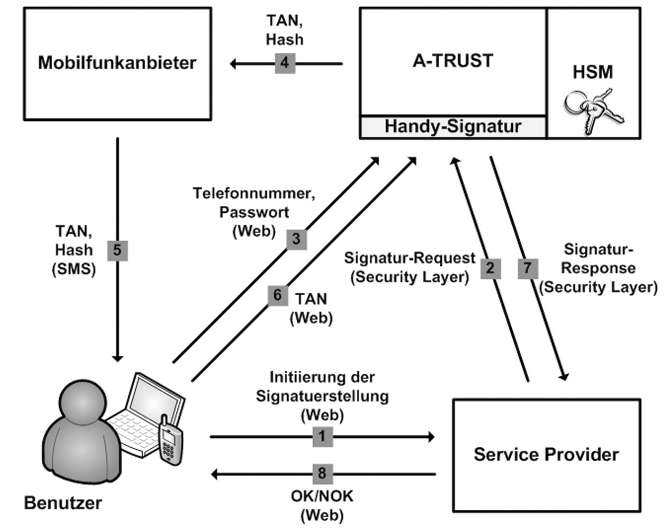
\includegraphics[width=\textwidth]{Abbildungen/Ablauf_Handy-Signatur.png}
    \caption{Schematischer Ablauf der Handy-Signatur \cite[S.~3]{mobQes}}
    \label{fig:HandySignaturablauf}
\end{figure}

Dabei ist zu beachten, dass dieser Vorgang nicht vom gleichen Endgerät ausgeführt werden soll, welches die SMS erhalten hat, da sonst keine \emph{qualifizierte} elektronische Signatur erstellt werden kann. Durch die Verwendung von Smartphones kann dies nicht sichergestellt werden, lediglich eine Belehrung des Benutzers kann erfolgen. Das Sicherheitskonzept der Anwendung basiert auf der Kombination von üblicher Passwortauthentifizierung und der \emph{Out-Of-Band Authentifizierung} als zweitem Faktor. Der Zugriff auf den \emph{privaten Schlüssel} zur Signaturerstellung muss also erstens durch ein Passwort und zweitens durch den separaten Kanal des Mobilfunknetzes, autorisiert werden. Die eigentliche Signaturerstellung wird von A-Trust in einem zentralem HSM\footnote{Hardware Sicherheits-Modul} vorgenommen, welches die kryptographischen Schlüssel des Benutzers sicher verwahrt. Die Schlüssel sind im HSM gegen direkten Zugriff abgesichert und können nur nach einer erfolgreichen Authentisierung des Benutzers verwendet werden.
\subsubsection{Vorteile}
Der Vorteil der Anwendung, gegenüber der Verwendung der Chipkarte (Bürgerkarte), ist die Verwendung des SMS-TAN als Authentifizierungsverfahren, statt eines Kartenlesegerätes am Computer des Benutzers. Somit soll eine maximale Verfügbarkeit der Anwendung sichergestellt werden, da die SMS-TAN von beliebigen Mobiltelefonen mit SIM-Karte empfangen werden kann. Außerdem bietet die \emph{Out-Of-Band Authentifizierung} einen zusätzlichen Schutz, falls der Computer des Benutzers kompromittiert sein sollte. Außerdem kann die Signaturerstellung in einer kontrollierten Umgebung stattfinden und somit auch einfacher und effizienter abgesichert werden.
\subsubsection{Nachteile}
Genau in der Tatsache, dass der Authentifizierungscode über eine SMS empfangen wird, liegt auch der größte Nachteil des Verfahrens. Während man eine Chipkarte gewohnheitsmäßig sicher verwahrt und der Zugriff darauf nur über spezielle Hardware mit einem PIN geschehen kann, ist das Mobiltelefon ein Alltagsgegenstand. Des weiteren ist nicht das Endgerät selbst für den Empfang des Authentifizierungscodes zuständig, sondern die Mobiltelefonnummer welche über die SIM-Karte beim Telekomunikationsdienstleister hinterlegt ist. Da die Mobiltelefonnummer kein sicheres Merkmal von Besitz ist, bekommt das Passwort welches zur Anmeldung im Online-Portal genutzt wird eine hohe Bedeutung. Wer Zugriff auf die Mobiltelefonnummer und das Zugangspasswort erlangt, hat die Möglichkeit im Namen dieser Person rechtskräftige Verträge abzuschließen. Mit modernen Smartphones ist es zudem auch möglich, sowohl die Web-Schnittstelle aufzurufen, als auch die SMS mit der TAN zu empfangen. Somit wird das Sicherheitsniveau der separaten Kanäle wieder reduziert. Zusätzlich ist die Trennung der Kanäle ein Nachteil für den Benutzer, da er die Anwendung nicht vom Smartphone benutzen kann sondern diese von einem Computer ausführen muss.

\subsection{Aktuelle Entwicklungen}\label{sec:scWorkshop}
Neuste Entwicklungen im Bereich der \textit{Handy-Signatur} ermöglichen auch alternative Authentifizierungsverfahren zur ursprünglich verwendeten \textit{SMS-TAN}, wie auf dem diesjährigen \textit{29. Smartcard Workshop} vorgestellt. Herbert Leitold und Daniel Konrad stellen im Beitrag \textit{Qualified remote signatures - Solutions, ITS certification, and use} \cite{scWorkshop} die aktuellsten Authentifizierungsverfahren der \textit{Handy-Signatur} im Kontext der \textit{eIDAS}-Verordnung dar. Durch die Prominenz der Smartphones im privaten Sektor werden aktuell zwei alternative Verfahren zur Authentifizierung implementiert:
\begin{description}[font=\rmfamily]
    \item[OTP mit QR Code:] Eine Clientanwendung wird für die verbreitetsten mobilen Betriebsysteme bereitgestellt, welche mit dem Benutzerkonto verknüpft ist. Diese Anwendung ermöglicht das Scannen eines QR Codes, welcher dem Benutzer durch die Web-Schnittstelle am Computer präsentiert wird, um sich zu authentisieren. Dieses Verfahren soll die Verwendung von zwei Geräten vorraussetzen.
    \item[Secure Hardware Element (SE):] Diese neuste Variante macht Gebrauch von den modernen, integrierten \textit{Secure Elements} in Smartphones. Das \textit{Secure Element} wird zur kryptographisch Kopplung des Benutzerkontos und des Signaturdienst genutzt und kann z.\,B. durch Biometrie freigeschaltet und anschließend zur Authentifizierung verwendet werden.
\end{description}
Aktuell ist das Standardverfahren die Authentifizierung mit einem \textit{Secure Element}, da es ein höheres Sicherheitsniveau bietet und unter bestimmten Vorraussetzungen auch sehr benutzerfreundlich ist. Jedoch setzt dieses Verfahren spezielle Hardware vorraus, welche sich noch nicht branchenübergreifend durchgesetzt hat.

\chapter{Authentifizierungsverfahren für die Fernsignatur}
In diesem Kapitel möchte ich ein Authentifizierungsverfahren der Handy-Signatur, die \textit{SMS-TAN}, näher analysieren und die Schwachstellen dieses Verfahrens im Kontext der serverseitigen mobilen Signatur aufzeigen. Wie bereits in Kapitel \ref{sec:Authentifizierung} dargestellt, handelt es sich bei der \textit{SMS-TAN} um die am weitesten verbreitete Zwei-Faktor Authentifizierung\footnote{In Kombination mit der üblichen Passwortauthentifizierung}. Ebenfalls werde ich die Anforderungen an die Authentifizierungsverfahren, welche in modernen Fernsignaturanwendungen eingesetzt werden, formulieren und sich eignende Authentifizierungsverfahren aufzeigen.
\section{Problematik der SMS-TAN}\label{sec:smstan-problematik}
Die \textit{SMS-TAN} ist ein Authentifizierungsverfahren, welche zur Kategorie der Authentifizierung durch Besitztum gehört. Um dieses Verfahren verwenden zu können muss der Benutzer seine Mobiltelefonnummer im Vorfeld beim Service-Provider registrieren und anschließend, wie in Abbildung \ref{fig:SMS-TAN_Registrierung} dargestellt, bestätigen. Jedoch setzt die österreichische Handy-Signatur einen komplexeren Registrierungsprozess um als es in Abbildung \ref{fig:SMS-TAN_Registrierung} dargestellt ist, da der Benutzer eine amtliche Registrierungsstelle aufsuchen oder von seiner bereits registrierten Bürgerkarte gebraucht machen muss. Somit wird die Mobiltelefonnummer, welche die \textit{SMS-TAN} empfängt, direkt an einen registrierten Bürger geknüpft. Das stellt die Grundlage der \emph{qualifizierten} elektronischen Signatur her. Die Transaktionsnummer (TAN) wird für genau eine Anwendung generiert und an den Benutzer, via SMS an sein Mobiltelefon, gesendet. Anschließend kann der Benutzer die TAN auslesen und sie innerhalb einiger Minuten beim Service-Provider\footnote{Google, Amazon, A-Trust, etc. - Meist über eine Web-Schnittstelle} eingeben um sich zu authentifizieren. Die \textit{SMS-TAN} wird in den aller meisten Fällen als Zwei-Faktor Authentifikation zusammen mit einem Passwort verwendet \cite{fido17}. Der typische Use-Case dieses Verfahrens sieht vor, dass der Benutzer sich erst mit einem Passwort authentifiziert bevor er eine SMS mit dem TAN zugesendet bekommt. Somit fungiert die \textit{SMS-TAN} als Einmal-Passwort und wird über den separaten Kanal des Mobilfunknetzes vom Benutzer empfangen. Abbildung \ref{fig:SMS-TAN} zeigt schematisch den Ablauf einer generischen Zwei-Faktor Authentifizierung mit Passwort und \textit{SMS-TAN}. Die Abläufe der Registrierung und der Authentifizierung unterscheiden sich nur im ersten Schritt und bieten dem Benutzer somit eine einfache Methode sich zusätzlich gegen unautorisierte Zugriffe abzusichern. Besonders die \textit{SMS-TAN} als Authentifizierungsverfahren erfuhr eine große branchenübergreifende Adaption, nicht zuletzt da Mobiltelefone und Smartphones sehr weit verbreitet sind. Nach angaben der Bitkom besitzen im Jahr 2017 78 Prozent aller Deutschen ein Smartphone \cite{bitkomMob} und die Tendenz ist steigend.

Die \textit{SMS-TAN} soll durch das Empfangen mit dem Mobiltelefon das Besitztum des Benutzer verifizieren und somit ein erhöhtes Sicherheitsniveau gegenüber der einfachen Passwortauthentifizierung bieten. In der Theorie trifft dies auch zu, jedoch stellt der Übertragunskanal, die verschiedenen Möglichkeit eine SMS zu empfangen und das Endgerät des Benutzers die Sicherheitseigenschaften des Verfahrens in Frage, insbesondere im Kontext der serverseitigen mobilen Signatur.
\begin{figure}[htbp]
    \centering
        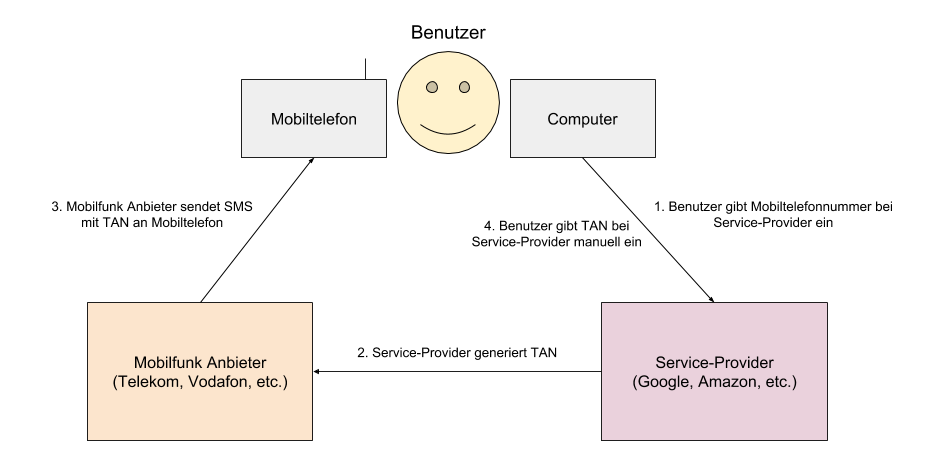
\includegraphics[width=\textwidth]{Abbildungen/Ablauf_SMS-TAN_Registrierung.png}
    \caption{Schematischer Ablauf der SMS-TAN Registrierung}
    \label{fig:SMS-TAN_Registrierung}

    \centering
        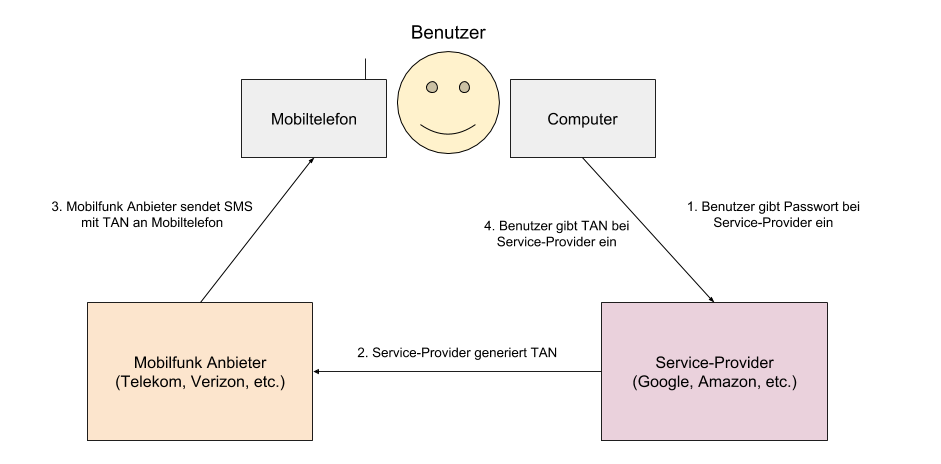
\includegraphics[width=\textwidth]{Abbildungen/Ablauf_SMS-TAN.png}
    \caption{Schematischer Ablauf der SMS-TAN Authentifizierung}
    \label{fig:SMS-TAN}
\end{figure}
\clearpage

\subsection{Mobiltelefonnummer als Merkmal von Besitz}
Mit der Registrierung einer Mobiltelefonnummer beim Service-Provider, z.\,B. A-Trust GmbH, soll ein Authentifikationsfaktor geschaffen werden, mit dem der Benutzer durch den Empfang einer \textit{SMS-TAN} den Nachweiß über den Besitz eines Mobiltelefons erbringen kann. Dieses Verfahren basiert somit auf dem Merkmal des Besitztums, jedoch ist die Mobiltelefonnummer, welche die \textit{SMS-TAN} empfängt, nicht direkt an das Gerät des Benutzer gekoppelt sondern an dessen SIM Karte. Mit der Evolution von ``einfachen'' Mobiltelefonen zu Smartphones ist auch das Risiko für Anwendungen wie der \textit{SMS-TAN} gestiegen. Der Grund dafür ist die zunehmende Vernetzung verschiedenster Geräte wie Smartphones, Tablets, Laptops und Computern. Es ist heutzutage möglich seine SMS nicht nur über das eigentliches Mobiltelefon zu empfangen, sondern diese an beliebige weitere Geräte und Dienste weiterzuleiten. Zusätzlich erlauben manche Mobilfunkanbieter die Verwendung von mehreren SIM Karten für eine Mobilfunknummer \cite{tmobileMultiSim}. Somit ist der Faktor Besitztum nicht mehr zweifelsfrei durch die Mobiltelefonnummer gegeben und das Sicherheitsniveau des Authentifizierungsverfahrens sinkt erheblich.

Ein wesentlicher Angriffsvektor auf den Benutzer ist die Mobiltelefonnummer selbst. Ein Angreifer muss keinen physischen Zugriff auf das Mobiltelefon haben um einen Angriff durchzuführen, da die Nachricht welche die TAN enthält an die Telefonnummer gerichtet ist und nicht an das Gerät selbst. Somit könnte ein Angreifer z.\,B. durch \emph{Social Engineering} den Mobilfunkbetreiber überzeugen die Mobiltelefonnummer auf einer neuen SIM Karte zu aktivieren. Diese Vorgehen wir auch \emph{SIM Hijacking} oder \emph{Port-Out Scam} genannt. Selbst T-Mobile warnt auf ihrer offiziellen Seite vor diesem Vorgehen \cite{telekomPortOut}. Der Angreifer gibt sich in diesem Szenario als der Benutzer beim Support des Netzbetreibers aus und behauptet die SIM Karte verloren zu haben, sodass die Telefonnummer auf eine neue SIM Karte überschrieben wird\footnote{Beispielhafte Erfahrung hier zu lesen: https://www.ftc.gov/news-events/blogs/techftc/2016/06/your-mobile-phone-account-could-be-hijacked-identity-thief}. Diese Art von Angriff unterstreicht die Problematik der \textit{SMS-TAN} als Authentifizierungsverfahren durch Besitz. Es liegt in der Verantwortung des Netzbetreibers die Telefonnummer des Benutzers zu verwalten und somit ist diese kein Beweis von Besitz des Benutzers über das Mobiltelefon. Für Angreifer wird es zunehmend einfacher die Mobilfunkbetreiber von einer gefälschten Identität zu überzeugen, da eine Vielzahl von personenbezogenen und vertraulichen Daten bereits durch Hacking-Angriffe auf große Unternehmen wie Equifax\footnote{https://www.ftc.gov/equifax-data-breach} zugänglich gemacht worden sind. Ebenfalls sind Angreifer aus den Reihen der Mobilfunkbetreiber möglich, da diese direkten Zugriff auf die Rufnummerverwaltung ihrer Kunden haben.

\subsection{Mobiltelefon}
Das Mobiltelefon und insbesondere das Smartphone als Weiterentwicklung sind aus dem heutigen Alltag nicht mehr wegzudenken. Das Smartphone ermöglicht gleichzeitig die Telefonie und den SMS Empfang aber auch den Zugriff auf multimediale Inhalte wie Musik, Videos, Spiele und Apps über das Internet. Insbesondere die Apps sind ein Risikofaktor für die Authentifikation via \textit{SMS-TAN}. Während andere Gegenstände wie die Bankkarte, welche zur Authentifikation genutzt werden, üblicherweise sicher aufbewahrt werden ist das Mobiltelefon ein Alltagsgegenstand und somit vielen Angriffsvektoren ausgesetzt. Besonders kritisch ist die Installation von Apps auf dem Smartphone, welche Zugriff auf die SMS haben\footnote{Der Zugriff muss in den meisten Fällen jedoch explizit gewährt werden}, da diese eine \textit{SMS-TAN} auslesen und an einen potenziellen Angreifer weiterleiten könnten. An dieser Stelle muss der Benutzer äußerst vorsichtig mit der Vergabe von Rechten an Apps sein, da sonst nur eine schädliche App auf dem Gerät des Benutzers das Sicherheitskonzept der \textit{SMS-TAN} untergraben könnte.

Ebenfalls problematisch ist die Aufhebung der separaten Kanäle durch Smartphones. Da es möglich ist den Web-Service des Service-Providers auch über das Smartphone aufzurufen besteht keine Trennung mehr zwischen der Passwortauthentifizierung über das Internet und dem Empfang der \textit{SMS-TAN} durch das Smartphone. Beide Komponenten der Zwei-Faktor Authentifizierung werden somit durch das selbe Endgerät verarbeitet. Infolge dessen muss nur ein Gerät, beispielsweise durch Keylogger, kompromittiert sein um das Sicherheitskonzept der Authentifikation zu durchbrechen. Es handelt sich grundsätzlich auch nicht um eine ``reine'' Out-Of-Band Authentifizierung, da die \textit{SMS-TAN} nur über den separaten Kanal des Mobilfunknetzes empfangen wird jedoch ebenfalls über eine Web-Schnittstelle an den Service-Provider gesendet wird.

Diese Eigenschaften in Verbindung mit der Möglichkeit die SMS an andere Geräte wie den Computer weiterzuleiten eröffnen eine Vielzahl von Angriffsvektoren auf die Zwei-Faktor Authentifizierung mit Passwort und \textit{SMS-TAN}. Das Mobiltelefon sollte für den Gebrauch von \textit{SMS-TAN} idealerweise kein Smartphone sein damit die Risikofaktoren der schädlichen Apps und der Zugriff auf die Web-Schnittstelle unterbunden werden. Falls doch ein Smartphone zur Authentifikation genutzt wird muss der Benutzer sich im klaren über die Vertrauenswürdigkeit der installierten Apps sein und die \textit{SMS-TAN} nicht über das selbe Gerät eingeben über das er die SMS empfangen hat.
\subsection{Mobilfunknetzwerk}
Heutzutage besteht das Mobilfunknetz aus einer Kombination von drei verschiedenen Technologien, welche aufeinander aufbauen:
\begin{enumerate}
    \item Global System Mobile (GSM / 2G)
    \item Universal Mobile Telecommunications System (UMTS / 3G)
    \item Long Term Evolution (LTE / 4G)
\end{enumerate}
GSM wurde von der \textit{European  Telecommunications  Standards  Institute (ETSI)} in den 1980er Jahren standardisiert. Es wurde absichtlich mit schwacher Verschlüsselung entwickelt, da zu der Zeit diverse europäische Regierungen eine Hintertür zu den Nachrichten haben wollten \cite{mobileSec}. Teile der Spezifikation von GSM wurden geheim gehalten und nur unter Geheimhaltungsverträgen an Industriepartner weitergegeben. GSM sieht außerdem keine Authentifikation der Funkstation gegenüber dem Mobiltelefon vor, was zur Folge hat, dass eine kompromittierte oder gefälschte Funkstation zum Abfangen von Nachrichten genutzt werden kann \cite[S.\,202]{komSec13}. Im Jahr 2000 wurde der Nachfolger UMTS durch das \textit{3rd Generation Partnership Project (3GPP)} standardisiert und kurze Zeit später kommerziell eingeführt. Verbesserungen dieses Standards gegenüber GSM waren die Authentifikation im Funknetz sowie stärkere kryptographisch Algorithmen \cite[S.\,203]{komSec13}. Aufbauend auf den vorhergegangen Architekturen wurde LTE entwickelt und circa 2010 eingeführt.

Moderne Mobiltelefone implementieren alle drei Standards um einen guten Empfang in diversen Situationen gewährleisten zu können. Problematisch ist jedoch die Verschlüsselung von 2G, denn diese basiert auf der \emph{A5 Algorithmenfamilie} \cite{mobileSec}. Es gibt eine Vielzahl von Varianten des A5 Algorithmus wie den A5/0 (Null Algorithmus), A5/1 und A5/2. Diese unterscheiden sich in ihrer Sicherheit, wobei keiner dieser Algorithmen nach modernen Standards sicher ist. Besonders kritisch ist die Version A5/0, welche die Daten unverschlüsselt sendet. Somit ist 2G das schwächste Glied in der Kette und ermöglicht es prinzipiell SMS Nachrichten abzufangen oder mitzulesen. So ist mit moderner Hardware sogar für Privatpersonen möglich einen \textit{Man-in-the-Middle} Angriff im GSM Netzwerk durchzuführen \cite[S.\,202]{komSec13}.

Ein weiterer Angriffsvektor ist das \textit{Signalling System} (SS7), da dessen Übertragungskanäle nicht kryptographisch geschützt sind \cite[S.\,202]{komSec13}. Das SS7 ist eine komplexe Sammlung von Protokollen welche in Telekommunikationsnetzen eingesetzt wird. Durch das SS7 können Angriffe auf den Mobilfunknutzer durchgeführt werden, wie eine Analyse der \textit{Security Research Labs} zeigt. Die \textit{Security Research Labs} aus Berlin weisen in einer Präsentation auf dem \textit{Chaos Computer Congress} auf die Schwächen des SS7 hin. So soll es möglich sein ein Mobiltelefon aufzuspüren, Nachrichten abzufangen oder Denial of Service Attacken durchzuführen \cite{cccMob}. Eine detaillierten Analyse der \textit{Security Research Labs} am Beispiel der Deutschen Netzbetreiber zeigt, dass es in einigen 2G Netzen möglich ist Nachrichten abzufangen \cite{srlMobSec}.

Durch die aufgeführten Defizite des Mobilfunknetzes als Übertragungskanal für Einmal-Passwörter ist eine sichere Zustellung der \textit{SMS-TAN} nicht gewährleistet.
\subsection{Mobilfunknetzbetreiber}
Ebenfalls ist ein Angriff auf den Benutzer auf der Ebene des Mobilfunknetzbetreibers zu denken. Die Verschlüsselung von GSM agiert nur in der Übertragung von der Funkstation bis zum Endgerät, welches die SMS empfängt. Die gesendeten Daten werden jedoch auch innerhalb der Infrastruktur des Netzbetreibers übertragen. Die dort eingesetzten Sicherheitsmaßnahmen sind nicht in der GSM Spezifikation festgelegt und somit unbekannt. Somit besteht die Möglichkeit, dass die SMS bereits durch den Mobilfunknetzbetreiber abgefangen oder mitgelesen wird. Auch wenn dieses Szenario unwahrscheinlich erscheint ist anzunehmen, dass ein solches Angriffsszenario durchführbar ist.

\subsection{Zusammenfassung}
Die \textit{SMS-TAN} als Authentifizierungsverfahren ist durch ihre Zugänglichkeit für den Benutzer und das erhöhte Sicherheitsniveau gegenüber der einfachen Passwortauthentifizierung eine beliebte Wahl der Zwei-Faktor Authentifizierung. So findet dieses Authentifizierungsverfahren viel Verwendung in Anwendungen, welche eine \emph{starke Authentifikation} erfordern. Beispiele für diese Anwendungsbereich sind Online-Banking, Online-Shopping und die österreichische \textit{Handy-Signatur}. Die der SMS zugrunde liegende Technologien und die Tatsache, dass es sich beim Mobiltelefon um einen Alltagsgegenstand handelt, stellt die absolute Sicherheit dieses Authentifizierungsverfahrens jedoch in Frage. Ebenfalls stellen die umfangreichen Anwendungsmöglichkeiten der Smartphones ein Sicherheitsrisiko für die Authentifizierung via \textit{SMS-TAN} dar. Smartphones sind anfällig für Schadsoftware und bieten dazu die Möglichkeit die Authentifizierung auf einem einzigen Endgerät durchzuführen, was wiederum die Separation der Kanäle gänzlich unterbindet. Ebenfalls zeigen sich Defizite in den Konzepten der Authentifizierung mit Besitz durch die \textit{SMS-TAN} und der Mobilfunknetze heraus. So sind bereits Angriffe durchgeführt worden, welche den Faktor des Besitzes umgangen haben oder es technisch ermöglichen die Nachrichten abzufangen und mitzulesen.

Ingesamt bietet die SMS \emph{keine} optimale Umgebung für eine Authentifikation per Einmal-Passwort, da das Engerät welches die SMS empfängt leicht kompromittiert werden kann und der Übertragungsweg nicht hinreichend abgesichert ist, wie in Tabelle \ref{table:AngriffsvektorenSMSTAN} zusammengefasst. Aus diesem Grund möchte ich im folgenden Kapitel alternative Authentifizierungsverfahren und ihre Kombinationen evaluieren.
\begin{table}[htbp]
    \begin{tabularx}{\textwidth}{ llX }
        \toprule
        Komponente & Angriffsvektor & Beschreibung  \\
        \midrule
        Mobiltelefonnummer & SIM Hijacking & Angreifer registriert die Telefonnummer auf eine neue SIM \\
        Mobiltelefonnummer & Weiterleitung & Durch das Weiterleiten der SMS können diverse weitere Sicherheitslücken ausgenutzt werden \\
        Mobiltelefon & Unbefugter Zugriff & Mobiltelefon als Alltagsgegenstand evtl. nicht ausreichend vor Zugriff gesichert \\
        Smartphone & Schadsoftware & Malware auf dem Smartphone kann Zugriff auf SMS Nachrichten haben und diese weiterleiten; Verstärkt durch die Benutzung des Smartphones als einziges Gerät \\
        Mobilfunknetz & GSM & Verschlüsselung der Nachricht nicht garantiert sicher \\
        Mobilfunknetz & SS7 & Abfangen von Nachrichten durch Schwachstellen im Protokoll in Verbindung mit der schwachen GSM Verschlüsselung \\
        Mobilfunknetz & Betreiber & Sicherheitsmaßnamen der Betreiber-internen Datenverarbeitung unbekannt \\
    \end{tabularx}
    \caption{Liste der Angriffsvektoren auf die \textit{SMS-TAN}}
    \label{table:AngriffsvektorenSMSTAN}
\end{table}
\clearpage

\section{Anforderungen}
Die Anforderungen an ein Authentifizierungsverfahren im Kontext der serverseitigen mobilen (Fern-)Signatur sind in erster Linie Sicherheitsanforderungen, jedoch spielen die Kategorien Benutzerfreundlichkeit und technische Komplexität auch eine Rolle. Die Verfahren müssen von einem Benutzer ausgeführt werden von dem anzunehmen ist, dass er kein technisches Hintergrundwissen hat. Somit müssen die Verfahren sowohl den Anforderungen an das Sicherheitsniveau als auch an die Benutzerfreundlichkeit und Umsetzbarkeit genügen. 

Aus Kapitel \ref{sec:eidas} lässt sich ableiten, dass der Zugriff auf die sicheren Signaturerstellungseinheiten (SSEE) besonderen rechtlichen Anforderungen genügen muss. So formuliert die \textit{eIDAS} Richtlinie, dass der Zugriff nur durch Mittel welche unter alleiniger Kontrolle des Benutzers stehen durchgeführt werden darf. Die für die Signaturerstellung notwendigen Authentifizierungsverfahren müssen diese Eigenschaft also wiederspiegeln, insbesondere weil die Fernsignatur impliziert dass der Benutzer keinen physische Zugriff auf die SSEE und die kryptographischen Schlüssel hat. Folglich müssen die Authentifizierungsverfahren eine starke Bindung an den Benutzer selbst haben um diesen eindeutig zu identifizieren. Ebenfalls sollte ein Authentifizierungsverfahren nicht, durch die unsachgemäße Anwendung des Benutzers, umgangen werden können (Bsp: Post-Its mit Passwort am Bildschirm).

Weitere Vorteile eines Authentifizierungsverfahrens im Kontext der Fernsignatur könnten Eigenschaften sein, welche zur Verschlüsselung der kryptographischen Schlüssel genutzt werden können um einen direkten Zugriff auf das HSM / SSEE zu vermeiden. Im Falle der \textit{Handy-Signatur} werden die privaten Schlüssel, welche zur Signaturerzeugung herangezogen werden, zusätzlich durch das Benutzerpasswort verschlüsselt. Somit sind sie vor Zugriff mit dem Hauptschlüssel des HSMs abgesichert. 

\section{Prinzipielle Eignung von Authentifizierungsverfahren für die Fernsignatur}
Die alternativen Authentifizierungsverfahren müssen sich für den Anwendungsbereich der mobilen serverseitigen Signatur eignen. Die \textit{Handy-Signatur} ist ein Dienst, welcher von einer breiten Masse der Bevölkerung benutzt werden soll und eine \emph{starke Authentifikation} erfordert. Somit sind die Aspekte Benutzerfreundlichkeit, Komplexität und insbesondere Sicherheit von besonderer Bedeutung. In Kapitel \ref{sec:AuthentifizierungVergleich} wurden die Eigenschaften der verschiedenen Authentifizierungsverfahren bereits in diesen Kategorien verglichen.
\begin{description}[font=\rmfamily]
    \item[Benutzerfreundlichkeit:] Die Verfahren der Kategorie \emph{Biometrie} sind besonders Benutzerfreundlich, da der Benutzer zur Authentifizierung nur seine körperlichen Merkmale braucht. \emph{Besitz}-basierte Verfahren hingegen erfordern vom Benutzer die Anschaffung und die sichere Verwahrung des Gegenstandes (z.\,B. Security Key). Jedoch existieren auch Verfahren welche auf bereits vorhanden Gegenständen basieren, wie die Chipkarte oder das Smartphone.
    \item[Komplexität:] Um eine hohe Verfügbarkeit des Authentifizierungsverfahrens für den Endbenutzer sicher zu stellen, sollte das Verfahren gegenüber dem Benutzer über eine geringe Komplexität verfügen. Das bedeutet, dass der Benutzer intuitiv und mit keinen bis wenigen Hilfsmittel eine Authentifizierung durchführen kann. Ebenfalls sollte das Verfahren auch für ``nicht Technik-Affine'' benutzbar sein. Die technische Komplexität spielt hier eine zweitrangige Rolle, ist jedoch ebenfalls ein wichtiges Kriterium da die benötigte Hardware (z.\,B. Iris-Scanner) möglicherweise sehr selten in Consumer-Produkten vorzufinden ist.
    \item[Sicherheit:] Das Verfahren soll die \textit{SMS-TAN} und somit die Schwächen dieses Authentifizierungsverfahrens ersetzen. Es ist also ein Verfahren gesucht, welches sicherer ist als die SMS-TAN. Die Defizite im Übertragungsweg und im Gerät, welches die SMS empfängt, müssen somit umgangen werden.
\end{description}
Tabelle \ref{table:Sicherheit} bietet eine Übersicht aller gängigen Authentifizierungsverfahren aus welcher die Verfahren \textit{Time-based One-Time Passwörter} und \textit{Universal Second Factor} anhand ihrer Eignung ausgewählt wurden.

Das \textit{Time-based One-Time Passwört} eignet sich besonders gut da keine Übertragung an das mobile Gerät, mit Ausnahme der initialen Geheimnisvereinbarung, stattfinden muss. Somit sind die Schwächen der \textit{SMS-TAN} in Hinsicht auf den Übertragungskanal umgangen. Ebenfalls kann man mit höherer Sicherheit sagen, dass das Gerät auf welchem der Passwortgenerator ausgeführt wird im Besitz des Benutzers ist, da es nachträglich nicht möglich ist einen zweiten Passwortgenerator zu initialisieren. Jedoch ist es möglich bei der Einrichtung des \textit{Time-based One-Time Passwört} mehrere Geräte zu initialisieren. Durch das Sandboxing von Anwendungen ist ebenfalls ein Zugriff durch dritte Anwendungen unterbunden. Zudem ist das Verfahren Benutzerfreundlich und sehr übersichtlich was die technische Komplexität angeht (wie im nächsten Kapitel dargestellt).

Einen ebenfalls hohen Sicherheitsstandard bietet der \textit{Universal Second Factor}, welcher es dem Benutzer ermöglicht sich auch durch Besitztum zu authentifizieren. Dieses Verfahren basiert auf kleinen kryptographischen Geräten, welcher zur Authentisierung benutzt werden können. Anders wie das \textit{Time-based One-Time Passwört} verwendet dieses Verfahren ein Public-Key-Kryptographiesystem, wobei die privaten Schlüssel sicher im Gerät gespeichert wird. Diese Eigenschaft macht es unmöglich ein zweites Gerät mit den selben Eigenschaften herzustellen oder zu kopieren, somit hat dieses Verfahren einen bedeutenden Vorteil gegenüber anderen Authentifizierungsverfahren durch Besitztum. Ebenfalls ist es nicht möglich Software oder ähnliches auf diesem Gerät auszuführen, was Malware ausschließt. Der \textit{Universal Second Factor} verwendet zur Authentifizierung ein \textit{Zero Knowledge Protokoll} durch ein Challenge-Response Vorgang, welches Man-In-The-Middle Angriffe unterbinden kann. Dieses Verfahren ist auch für den Benutzer einfach zu bedienen, da er in der Regel nur ein USB-Stick ähnliches Gerät anschließen und einen Knopf berühren muss. Diese simple Methodik wird durch den \textit{U2F} Standard der \textit{FIDO Alliance} ermöglicht.

Biometrische Verfahren sind in der Regel am benutzerfreundlichsten wie in Kapitel \ref{sec:AuthentifizierungVergleich} beschrieben. Da viele moderne Smartphones mit zuverlässigen Fingerabdrucksensoren ausgestattet sind eignen sich diese hervorragend zur Authentifizierung eines Benutzers. Der Fingerabdruck des Menschen ist bekanntlich einmalig und kann eine Person deshalb zweifelsfrei identifizieren. Biometrische Authentifizierungsverfahren durch Fingerabdrücke können ähnlich wie der \textit{Universal Second Factor} durch ein Public-Key-Kryptosystem implementiert werden und von dessen Eigenschaften profitieren. So wird ebenfalls ein Challange-Response Protokoll verwendet um den Benutzer zu authentifizieren, dazu muss der Benutzer den Zugriff auf den privaten Schlüssel, welche auf dem Endgerät gespeichert sind, durch seinen Fingerabdruck gewähren. Die Implementierung eines solchen Systems, zusätzlich zur eigentlichen Webanwendung würde den Rahmen dieser Arbeit jedoch sprengen. Ebenfalls setzt eine solche Implementierung ein Smartphone mit Fingerabdruckscanner und sicherem Speicher vorraus. Durch die Verwendung eines Public-Key Kryptographiesystems ähnelt dieses Authentifizierungsverfahren sehr \textit{U2F}. Aus diesen Gründen wird die biometrische Authentifizierung im folgenden Kapitel nicht weiter evaluiert.

\chapter{Experimentelle Evaluation}
Sicherheitskritische Anwendung wie die \textit{Handy-Signatur} erfordern eine \emph{starke} Authentifizierung. Typischerweise wird eine solche Authentifizierung durch eine Zwei- oder Multi-Faktor Authentifizierung implementiert. Eine Kombination der in Kapitel \ref{sec:Authentifizierung} vorgestellten Authentifizierungsverfahren erhöht das Sicherheitsniveau einer Anwendung erheblich. In den meisten Fällen wird von Service-Providern eine Kombination von üblicher Passwortauthentifizierung und \textit{SMS-TAN} benutzt \cite{fido17}. Die \textit{SMS-TAN} ist wie in Kapitel \ref{sec:smstan-problematik} erläutert jedoch keine optimale Wahl für besonders gefährdete Anwendungsbereiche wie die \textit{Handy-Signatur}.

Im Folgenden möchte ich alternative Authentifizierungsverfahren evaluieren, welche die \textit{SMS-TAN} und ihre Schwächen ersetzen sollen. Als grundlegender ersten Faktor der Authentifizierung wird das Passwort beibehalten, da dieses sich etabliert hat und den Faktor des Wissens am besten repräsentiert. Aus diesem Grund werden Faktoren aus der Kategorie \emph{Wissen} hier nicht weiter betrachtet. Ziel dieser Evaluation ist es Erkenntnisse zu sammeln um die abschließende Eignung der Authentifizierungsverfahren für die Fernsignatur zu bestimmen. Zusammen mit den Erkenntnissen der vorhergegangenen Kapiteln lässt sich so eine fundierte Aussage über die Tauglichkeit in Sicherheit, Benutzerfreundlichkeit und Komplexität formulieren.

Die Implementierung der alternativen Authentifizierungsverfahren erfolgt \emph{prototypisch} auf Basis einer \textit{Ruby on Rails} Webanwendung in der Programmiersprache \textit{Ruby}. Weitergehende Informationen zu den benutzten Verfahren und Bibliotheken finden sich in den entsprechenden Kapiteln.

\section{Time-based One-Time Password (TOTP)}\label{sec:TOTP}
Das Time-based One-Time Password (Zeit-basiertes Einmal-Passwort), im Folgenden nur noch \textit{TOTP} gennant, ist eine Software-basiertes Authentifizierungsverfahren durch Besitztum. \textit{TOTP} basiert auf einem \textit{HMAC}\footnote{Hash-based message authentication code}-Einmal-Passwort Algorithmus (HOTP) und erzeugt zeitlich eingeschränkte Einmal-Passwörter. Ein Auszug aus dem RFC 6238 unterstreicht die Eignung des Verfahrens als Zwei-Faktor Authentifizierung für Transaktions-orientierte Webanwendungen:
\begin{quote}
    ``The proposed algorithm can be used across a wide range of network
    applications, from remote Virtual Private Network (VPN) access and
    Wi-Fi network logon to transaction-oriented Web applications.  The
    authors believe that a common and shared algorithm will facilitate
    adoption of two-factor authentication on the Internet by enabling
    interoperability across commercial and open-source implementations.'' \cite{rfc6238}
\end{quote}
Im Rahmen der \textit{Initiative For Open Authentication (OAUTH)} wurde das \textit{TOTP} entwickelt und soll einen branchenübergreifenden Standard definieren. Eine weit verbreitete Implementierung dieses Authentifizierungsverfahrens, auf Seiten des Benutzers, ist der \textit{Google Authenticator}.
\subsection{Funktionsweise}
Das \textit{TOTP} erweitert den \textit{HMAC}-Einmal-Passwort Algorithmus, jedoch benutzt \textit{TOTP} die UNIX-Zeit\footnote{Gangzahliger Wert in Millisekunden seit 01.01.1970} als variablen Faktor der Passwortgenerierung, statt einem Zähler. Für den Algorithmus werden folgende Werte benötigt:
\begin{itemize}
    \item $K$ : Geheimnis, welches zwischen Client und Server vereinbart wird
    \item $X$ : Zeitschritt in Sekunden (Standardwert $X = 30$)
    \item $T_0$ : UNIX-Zeit als Startwert der Zählung der Zeitschritte (UNIX-Epoche $T_0 = 0$)
    \item $T_a$ : Aktuelle UNIX-Zeit
\end{itemize}
Der Integer $T$ berechnet sich aus $T = (T_a - T_0) / X$ und gibt die Anzahl der Zeitschritte seit $T_0$ und der aktuellen Zeit an. Somit ist das \textit{TOTP} definiert als $TOTP = HOTP(K, T)$. Der \textit{HOTP} Algorithmus ist in RFC 4226\footnote{https://tools.ietf.org/html/rfc4226} definiert und kann in drei Grundschritte zusammengefasst werden:
\begin{enumerate}
    \item Generiere einen HMAC-SHA-1 Wert mit einem Zähler $C$: 
    \[
        HS = \textrm{HMAC-SHA-1}(K, C)
    \]
    \item Generiere einen 4-Byte langen String (Dynamic Truncation $DT$): 
    \[
        S_{bits} = DT(HS)
    \]
    \item Berechnen den \textit{HOTP}-Wert mit $S_{num}$ als Konvertierung von $S_{bits}$ in eine Ziffer und Digit = Anzahl der Ziffern des generierten Passworts:
    \[
        D = S_{num} \bmod 10^{\textrm{Digit}}
    \]
\end{enumerate}
\subsection{Eigenschaften}
Das \textit{TOTP} ist ein Software-basiertes Verfahren und benötigt deshalb eine Ausführungsumgebung. Für den Benutzer heißt das, dass er eine Client-Software installieren muss. Ein populäres Softwareprodukt wird von Google angeboten: Der \textit{Google Authenticator} ist eine Anwendung für Smartphones mit Android, iOS oder Blackberry Betriebssystem. Ebenfalls sind alternative Implementierungen für Smartphones und Desktopcomputer verfügbar (Authy, KeePassXC, 1Password). Die Service-Provider hingegen müssen eine API implementieren, welche zum RFC 6236 kompatibel ist. Ein Beispiel dafür ist die Bibiliothek \textit{ROTP}\footnote{https://github.com/mdp/rotp} in der Programmiersprache \textit{Ruby}. Die Gegenseitige Kompatibilität wird durch RFC 4226 (HOTP) und RFC 6236 (TOTP) sichergestellt.

Dieses Authentifizierungsverfahren eignet sich gut als Subsitution der \textit{SMS-TAN}, da ebenfalls ein Smartphone vom Benutzer genutzt werden kann. Jedoch werden nur Smartphones mit Android, iOS und Blackberry Betriebssystem unterstützt, infolge dessen können alte Mobiltelefone für dieses Verfahren nicht verwendet werden\footnote{Im Falle von \textit{Google Authenticator}}. Im Gegensatz zur \textit{SMS-TAN} ist keine Übertragung des Einmal-Passworts zum Endgerät notwendig, lediglich bei der Registrierung des Authentifizierungsverfahrens muss zwischen Client und Server ein Geheimnis vereinbart werden welches zur Passworterzeugung genutzt wird. Diese Eigenschaft umgeht die Schwächen der \textit{SMS-TAN} im Bezug auf den Übertragungskanal gänzlich. Durch App-Sandboxing ist ebenfalls kein Zugriff auf das Passwort durch andere Applikationen möglich, sodass sich insgesammt ein höheres Sicherheitsniveau ergibt. Das \textit{TOTP} eignet sich außerdem besser als Authentifizierung durch Besitz, da der physische Zugriff auf das Gerät, welches den Client ausführt, gegeben sein muss. Ein weitere Vorteil ist die Dauer der Gültigkeit der erzeugten Passwörter, denn diese sind in der Regel nur 30 Sekunden gültig und machen somit einen Angriff schwieriger. Für den Benutzer ergibt sich dadurch jedoch kein Nachteil, da er einfach das Passwort des darauf folgenden Intervalls nutzen kann.

\subsection{Sicherheit}
Die Sicherheit dieses Verfahrens hängt im Wesentlichen von der Speicherung des Geheimnisses ab, da dieses zur Erzeugnung von gültigen Passwörtern genutzt werden kann. Somit müssen die Geheimnisse sicher und verschlüsselt gespeichert werden. Ebenfalls muss die initiale Übertragung des Geheimnisses unbedingt über einen sicheren und verschlüsselten Kanal wie SSL geschehen, da sonst nicht gewährleisten werden kann dass nur der Benutzer das Geheimnis kennt. Das erfolgsversprechendste Angriffsszenario ist ein Brute-Force Angriff, da das Passwort meist nur aus 6 Ziffern besteht. Dieses lässt sich jedoch einfach unterbinden, indem die Eingabe auf eine geringe Anzahl an Versuchen beschränkt wird. Insgesammt ist die Sicherheit im direkten Vergleich zur \textit{SMS-TAN} höher, da die Passwörter nicht über den unsicheren Kanal des Mobilfunknetzwerks übertragen werden müssen und andere Anwendungen keinen Zugriff auf die Passwörter haben.

\subsection{Schwächen}
Wie bei allen Verfahren der Kategorie Authentifizierung durch Besitz ist dieses Authentifizierungsverfahren anfällig gegen Diebstahl. Beim Smartphone handelt es sich um ein Alltagsgegenstand der nicht zuverlässig gesichtert aufbewahrt wird. Es ist also in der Verantwortung des Benutzers das Smartphone ausreichend gegen unbefugten Zugriff, z.\,B. durch einen PIN, zu sichern. Ebenfalls stellen \textit{Man-In-The-Middle}-Angriffe ein Risiko für das Authentifizierungsverfahren dar. In so einem Angriffsszenario leitet der Angreifer den Benutzer auf eine gefälschte Seite und entlockt ihm so die Passwörter.

\subsection{Implementierung}\label{sec:TOTPImpl}
Dieses Kapitel dient zur Veranschaulichung einer simplen, jedoch effektiven Implementierung einer Multi Faktor Authentifizierung mit Zeitbasierten Einmal-Passwörtern. Als Grundlage dafür habe ich eine eine Webanwendung mit dem Framework \textit{Ruby on Rails}\footnote{https://rubyonrails.org/} gebaut und darauf aufbauend eine \textit{TOTP}-Authentifizierung, wie in Kapitel \ref{sec:TOTP} beschrieben, implementiert. Die Webanwendung soll es einem registrierten Benutzer ermöglichen Nachrichten zu erstellen und diese anschließend zu signieren. In der Webanwendung ist es einem Benutzer möglich sich mit Name, E-Mail und Passwort zu registrieren, wie in Abbildung \ref{fig:Authwebapp_login} gezeigt. Um sich jedoch erstmals in der Webanwendung anmelden zu können muss der Benutzer den Zugriff auf die angegebene E-Mail Adresse bestätigen indem er auf einen Link in einer initialen E-Mail klickt, welche er von der Webanwendung zugeschickt bekommt\footnote{Falls der Server keine Authentifiziung beim SMTP Server durchführen konnte, findet sich der Aktivierungslink in der Konsole.}. Anschließend hat der Benutzer Zugriff auf sein Konto. Um jedoch Zugriff auf die Signaturerstellung zu haben, muss der Benutzer jedoch zusätzlich den zweiten Faktor der Authentifizierung in den Kontoeinstellungen aktivieren, in diesem Fall das \textit{TOTP}. Um ein \textit{TOTP} zu aktivieren muss der Benutzer ein Haken in der entsprechenden Checkbox setzen und anschließend den ihm präsentierten QR-Code in einer Software seiner Wahl (hier mit \textit{Google Authenticator} getestet) auf einem zweiten Gerät scannen (siehe Abbildung \ref{fig:Authwebapp_qr}). Anschließend muss der Benutzer ein Einmal-Passwort, welches ihm z.\,B. vom \textit{Google Authenticator} generiert wird eingeben. Falls das Passwort nicht stimmt oder der Benutzer den Vorgang abricht wird keine \textit{TOTP} Authentifizerung aktiviert. Im Falle einer erfolgreichen Verifizierung durch den Server mithilfen eines asynchronen Aufrufes wird die Checkbox im aktivierten Zustand gelassen und der Benutzer kann durch eine finale Bestätigung das Authentifizierungsverfahren aktivieren. Die Initialisierung des \textit{TOTP} wird nocheinmal schematisch in Abbildung \ref{fig:totp-init} gezeigt. Ähnlich zur initialen Verifikation und Aktivierung des \textit{TOTP} ist die eigentliche Authentifizierung eines angemeldeten Benutzers mittels \textit{TOTP} zur Signaturerstellung durchzuführen, wie Abbildung \ref{fig:totp} darstellt.
\begin{figure}[htbp]
    \centering
        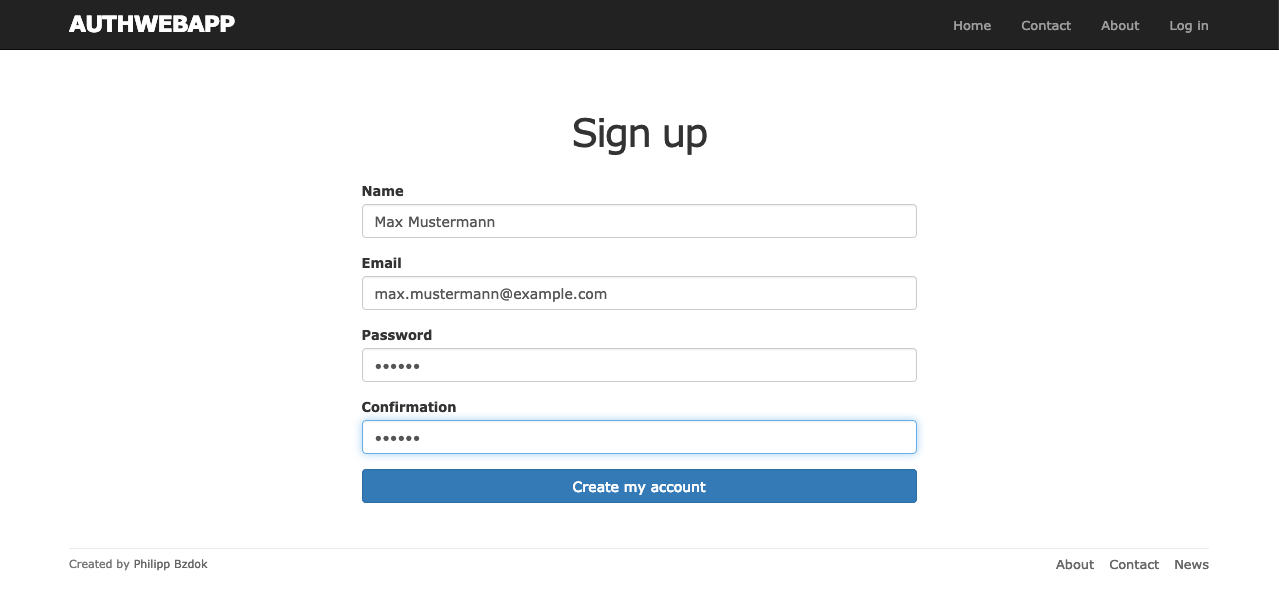
\includegraphics[width=\textwidth]{Abbildungen/Authwebapp_login}
    \caption{Anmeldeseite der Webanwendung}
    \label{fig:Authwebapp_login}
\end{figure}
\begin{figure}[htbp]
    \centering
        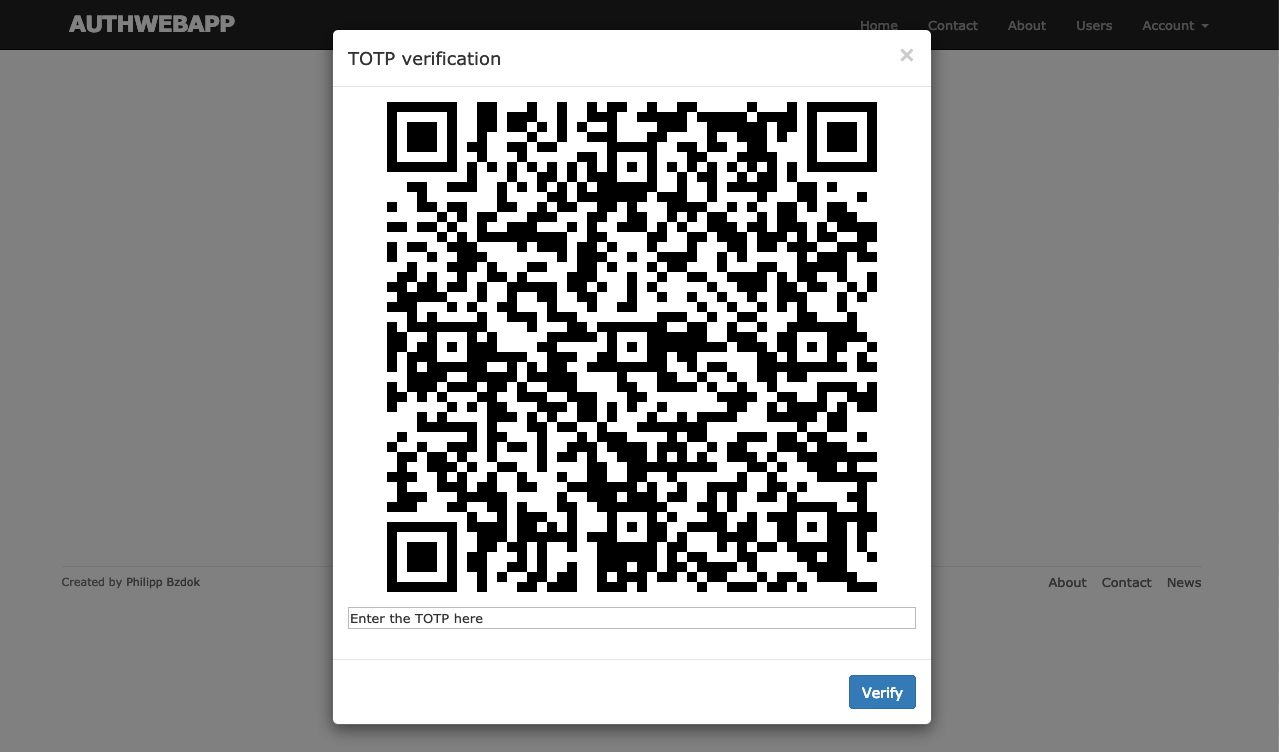
\includegraphics[width=\textwidth]{Abbildungen/Authwebapp_qr}
    \caption{QR-Code zur Aktivierung der TOTP Authentifizierung}
    \label{fig:Authwebapp_qr}
\end{figure}
\begin{figure}[htbp]
    \centering
        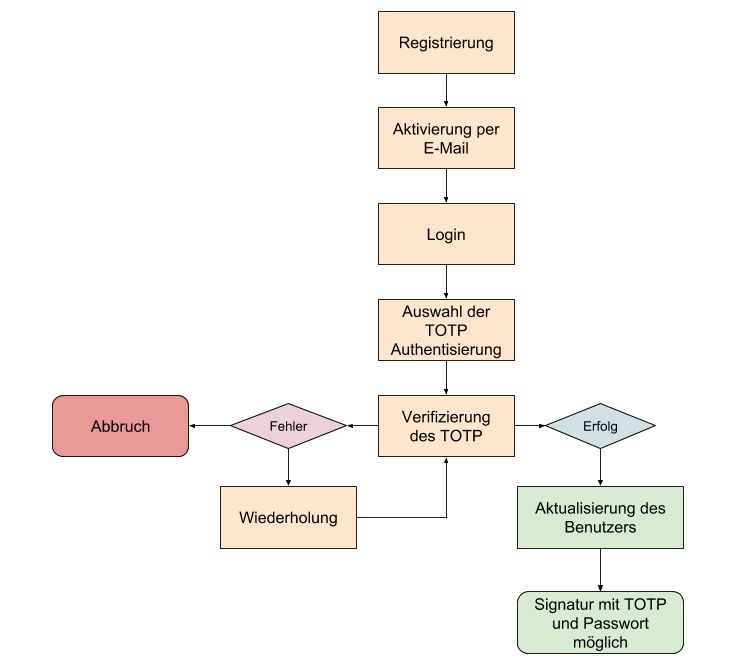
\includegraphics[width=\textwidth]{Abbildungen/Ablauf_TOTP_Initialisierung}
    \caption{Schematischer Ablauf der TOTP Initialisierung}
    \label{fig:totp-init}
\end{figure}
\begin{figure}[htbp]
    \centering
        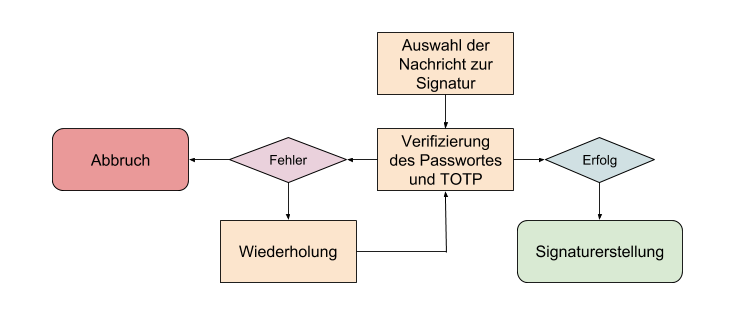
\includegraphics[width=\textwidth]{Abbildungen/Ablauf_TOTP}
    \caption{Schematischer Ablauf der TOTP Authentifizierung}
    \label{fig:totp}
\end{figure}
\clearpage

Da \textit{Ruby on Rails} eine \textit{Model-View-Controller} Architektur folgt stelle ich im Folgenden die relevanten Details meiner Implementierung innerhalb ihrer Komponenten dar:
\subsubsection{Model}
Das \textit{Model} bezieht sich auf die Entitäten der Webanwendung und beschreibt diese. Anhand der im \textit{Model} definierten Eigenschaften wird eine Datenbanktabelle erstellt. Im Falle des Benutzers sind dabei die Spalten aus Tabelle \ref{table:db-user} erstellt worden\footnote{Hierbei ist zu beachten, dass das \texttt{otp\_secret} nicht verschlüsselt gespeichert wird, da dies den Rahmen des Protoypen sprengen würde}.
\begin{table}[htbp]
    \begin{tabularx}{\textwidth}{ lX }
        \toprule
        Spalte & Beschreibung \\ 
        \midrule
        \texttt{name} & Name des Benutzers \\
        \texttt{email} & E-Mail des Benutzers \\
        \texttt{created\_at} & Erstellungsdatum des Benutzerkontos \\
        \texttt{updated\_at} & Aktualisierungsdatum des Benutzerkontos \\
        \texttt{password\_digest} & Hashwert des bei der Anmeldung angegebenen Passworts \\
        \texttt{actvation\_digest} & Hashwert eines E-Mail-Verifizierungs Tokens \\
        \texttt{activated\_at} & Zeitpunkt der Kontoaktivierung \\
        \texttt{totp\_activated} & Boolscher Wert ob TOTP Authentifizierung aktiviert ist \\
        \texttt{otp\_secret} & Wert anhand dessen eine TOTP Authentifizerung registriert und ausgeführt werden kann \\
        \bottomrule
    \end{tabularx}
    \caption{Datenbanktabelle - Benutzer}
    \label{table:db-user}
\end{table}

Das \textit{User Model} wird programmatisch definiert und erlaubt somit Validitätsprüfungen der Werte, bevor ein Benutzer in der Datenbank gespeichert wird. Konkret werden E-Mail Adressen einer Prüfung durch einen regulären Ausdruck unterzogen, die Existenz des Namens und Einschränkungen bezüglich der Passworteigenschaften geprüft. Ebenfalls lassen sich Beziehungen zu anderen \textit{Model}-Klassen definieren, so hat in dieser Implementierung das \textit{User Model} eine 1-n Beziehung zum \textit{Message Model}, welches die zu signierenden Nachrichten repräsentiert. Diese Eigenschaften des \textit{Models} sind dargestellt in Listing \ref{lst:User.rb-dsl}. Typisch an dieser Stelle für \textit{Ruby on Rails} ist die \textit{Domain Specific Language} (DSL), welche durch Metaprogrammierung in Ruby ermöglicht wird. Ebenfalls werden Funktionen im \textit{Model} implementiert, welche auf einer Instanz des Objektes zur Laufzeit agieren und somit die Anwendungslogik definieren. Ein Beispiel für solch eine Funktion, welche essenziel für die Anwendung ist, ist die Generierung eines \textit{TOTP}-Objektes und des dazugehörigen QR-Codes für die Initialisierung des Authentifizierungsverfahrens (siehe Listing \ref{lst:User.rb-createTOTP}). Dazu wurden die Ruby Bibiliotheken\footnote{Auch \textit{Gems} gennant} \textit{rotp - Ruby one-time-password}\footnote{https://github.com/mdp/rotp} und \textit{rqrcode - Ruby QR Code}\footnote{https://github.com/whomwah/rqrcode} verwendet. Die Grundlage für die Erstellung eines TOTP ist das Geheimnis welches zwischen Server und Client ausgehandelt wird. Die Erstellung eines solchen Wertes wird ebenfalls im \textit{Model} definiert, da jeder Benutzer einen eigenen Wert bekommt: \ruby{self.otp_secret = ROTP::Base32.random_base32} .Das \texttt{otp\_secret} wird bereits bei der Erstellung des Benutzerkontos generiert und gespeichert um eine unmittelbare Verifizierung eines \textit{TOTP} zu ermöglichen. Direkt nach der Erstellung des Kontos kann mit Hilfe des Geheimnisses eine \textit{TOTP}-Instanzvariable \ruby{ROTP::TOTP.new(otp_secret)} generiert werden (Zeile 4 in Listing \ref{lst:User.rb-createTOTP}) und anschließend der QR-Code im Frontend weiterverarbeitet werden. Die Instanzvariable der \textit{rotp} Bibliothek implementiert die nötigen Funktionen zur Erstellung und Verifizierung eines \textit{TOTP}. Die Verifizerung kann nun bei Bedarf auf der Objektinstanz des Benutzers aufgerufen werden, indem das Geheimnis herangezogen wird um eine \textit{rotp} Instanzvariable zu initialisieren. Dieses Vorgehen setzt in der Produktivumgebung eine sichere Speicherung des \texttt{otp\_secret} vorraus, da dieser genutzt werden kann um weitere Passwortgeneratoren zu initialisieren.
\begin{listing}[htpb]
    \begin{minted}{ruby}
        class User < ApplicationRecord
            has_many :messages, dependent: :destroy
            has_secure_password
        
            attr_accessor :remember_token, :activation_token, :reset_token, :totp
        
            before_create :create_activation_digest, :create_otp_secret
            before_save   :downcase_email
        
            validates :name, presence: true,
                            length: { maximum: 50 }
        
            VALID_EMAIL_REGEX = /\A[\w+\-.]+@[a-z\d\-.]+\.[a-z]+\z/i
            validates :email, presence: true,
                            length: { maximum: 255 },
                            format: { with: VALID_EMAIL_REGEX },
                            uniqueness: { case_sensitive: false }
        
            validates :password, presence: true,
                                length: { minimum: 6 },
                                allow_nil: true
            # [...]
        end
    \end{minted}
    \caption{\texttt{User.rb} - Definition der Eigenschaften in \textit{DSL}}
    \label{lst:User.rb-dsl}
\end{listing}
\begin{listing}[htpb]
    \begin{minted}{ruby}
        # [...]
        # Creates and assigns the totp object and returns the qr code
        def create_totp
          self.totp = ROTP::TOTP.new(otp_secret)
          RQRCode::QRCode.new(totp.provisioning_uri('AuthWebApp'), size: 8, level: :h)
        end
        # [...]
    \end{minted}
    \caption{\texttt{User.rb} - Funktion zur Generierung eines TOTP-Objektes}
    \label{lst:User.rb-createTOTP}
\end{listing}

Das \textit{Model} der zu signierenden Nachrichten fällt etwas simpler aus, da dieses keine Parameter für die Authentifizierung benötigt. Die wesentlichen Eigenschaften der Nachrichten beschränken sich auf die Beziehung zum Benutzer, den Inhalt und die Signatur. Tabelle \ref{table:db-message} veranschaulicht nochmal die Datenbanktabelle des \textit{Message Models}. Die Funktionen des \textit{Models} beschränken sich auf die Erstellung und Verifikation der Signatur und sind in Listing \ref{lst:Message.rb} aufgeführt. Die von den Funktionen erwarteten Parameter sind von der \textit{OpenSSL} Bibliothek\footnote{https://ruby-doc.org/stdlib-2.6.2/libdoc/openssl/rdoc/OpenSSL.html} von Ruby erzeugte Objekte welche ein RSA Schlüsselpaar mit Länge 2048 abbilden. Wichtig an dieser Stelle ist das Kodieren der von OpenSSL generierten Signatur in UTF-8, da die verwendete Datenbank SQLite 3 keine ASCII 8-Bit Kodierung unterstützt. Jedoch muss die ASCII 8-Bit Kodierung bei der Verifikation wiederhergestellt werden. Weitere Parametere benötigen den Funktionen nicht, da der Inhalt der Nachricht sowie die Signatur Teile der Message Instanz sind, welche aus der Datenbank gelesen werden.
\begin{table}[htbp]
    \begin{tabularx}{\textwidth}{ lX }
        \toprule
        Spalte & Beschreibung \\ 
        \midrule
        \texttt{content} & Inhalt der Nachricht \\
        \texttt{user\_id} & ID des zugehörigen Benutzers \\
        \texttt{created\_at} & Erstellungsdatum der Nachricht \\
        \texttt{updated\_at} & Aktualisierungsdatum der Nachricht \\
        \texttt{signature} & Signaturwert kodiert als UTF-8 String \\
        \bottomrule
    \end{tabularx}
    \caption{Datenbanktabelle - Message}
    \label{table:db-message}
\end{table}
\begin{listing}[htpb]
    \begin{minted}{ruby}
        class Message < ApplicationRecord
            belongs_to :user
            validates :user_id, presence: true
            validates :content, presence: true

            def sign_content(keypair)
                signature_ascii_8bit = keypair.sign_pss("SHA256",
                                                        content,
                                                        salt_length: :max,
                                                        mgf1_hash: "SHA256")
                self.signature = Base64.encode64(signature_ascii_8bit).encode('utf-8')
            end

            def verify_signature(keypair)
                decoded_signature = Base64.decode64(signature.encode('ascii-8bit'))
                keypair.public_key.verify_pss("SHA256",
                                            decoded_signature,
                                            content,
                                            salt_length: :auto,
                                            mgf1_hash: "SHA256")
            end
        end
    \end{minted}
    \caption{\texttt{Message.rb} - Funktionen des Message Models}
    \label{lst:Message.rb}
\end{listing}
\clearpage
\subsubsection{Controller und Routen}
Für den Zugriff auf das Model und dessen Funktionen sind die \textit{Controller} zuständig. Die \textit{Controller} steuern den Zugriff auf die \textit{Models} und die dazugehörigen \textit{Views}. Für die \textit{TOTP}-Verifikation wird anhand der URL eine Route bestimmt und vom \textit{Controller} verarbeitet. Listing \ref{lst:routes.rb} zeigt die definierten Routen. Die dort definierten Ressourcen sind meistens \textit{Models} und in der Datenbank hinterlegt, können jedoch auch temporäre Daten oder statische HTML Seiten sein. Des weiteren lassen sich die ausführbaren Operation, über die standard CRUD-Operationen\footnote{Create, Read, Update, Delete} hinaus, erweitern (z.\,B. \ruby{get '/signup', to: 'users#new'}) und / oder einschränken (z.\,B. \ruby{resources :messages, only: [:create, :destroy]}). Besonders wichtig für die Implementierung der \textit{TOTP} Authentifizierung ist die Erweiterung der User Ressource um die Funktionalität der Verifizierung. Dazu wird eine spezielle Route, basierend auf einem User definiert (siehe Listing \ref{lst:routes.rb}, Zeilen 11-13), welche die CRUD-Operationen um die Route \texttt{GET /users/:id/verify\_otp} ergänzt. Die Funktionalität dahinter wird im \textit{Controller} durch die Funktion \texttt{verify\_otp} definiert. Diese Funktion stellt die Kernfunktionalität der \textit{TOTP}-Authentifizierung, die Verifizierung dar. Im Gegensatz zu den restlichen Operationen für User bietet diese Operation keine \textit{View} an. Der Aufruf der Operation wird über \texttt{GET /users/:id/verify\_otp} getätigt und erwartet die Parameter \texttt{UserID} und \texttt{totp}. Aufrufe an diese URL prüfen immer ob der angegebene Benutzer existiert, ob die aktuelle Session aktiv ist und ob der Benutzer angemeldet ist um unauthorisierten Zugriff zu vermeiden. Listing \ref{lst:user-controller.rb-verify-otp} zeigt die Funktion welche beim Aufruf auf \texttt{GET /users/:id/verify\_otp} aufgerufen wird. Der Rückgabewert der Funktion bildet den Rückgabewert der Verifizierungsfunktion des \textit{User Models} (siehe Listing \ref{lst:user.rb-verify-otp}) auf ein JSON Objekt ab. Dieses JSON Objekt kann im Folgenden vom Frontend interpretiert werden. An dieser Stelle ist anzumerken, dass nur das \textit{TOTP} vom Browser zum Server übertragen werden muss und das Gerät welches das Passwort generiert keinerlei Verbindung braucht.

Die Signaturerstellung wurde über den Aufruf der Operation \texttt{/messages/:id/edit} implementiert. Der Aufruf leitet den Benutzer weiter an eine View, welche es ihm ermöglicht den Nachrichteninhalt zu sehen und zu signieren. Dabei wird ein Benutzer welcher keine Multi-Faktor Authentifizierung aktiviert hat auf sein Profil umgeleitet mit dem Hinweiß, dass eine Signatur nur mit Multi-Faktor Authentifizierung möglich ist. Falls ein weiteres Authentifizierungsverfahren für den Benutzer aktiv ist, so kann er dieses Verfahren verwenden um die Nachricht zu signieren (siehe Abb. \ref{fig:Authwebapp_sign_TOTP}). War die Authentifizierung des Benutzers via TOTP erfolgreich, so wird ein asynchroner Aufruf an die PUT Operation auf \texttt{/message/:id} getätigt und die wird Nachricht mit dem privaten Schlüssel des Benutzers signiert und gespeichert. Um einen Angriff auf diese zweite konsekutive Operation zu unterbinden wird bei der TOTP Authentifizierung ein Authentifizierungstoken generiert und in der Response returniert. Die konsekutive PUT Operation prüft anschließend die Gültigkeit des Tokens bevor die Nachricht signiert wird, wie in Listing \ref{lst:messages_controller.rb-update} dargestellt.
\begin{listing}[htpb]
    \begin{minted}{ruby}
        Rails.application.routes.draw do
            root 'static_pages#home'
            get '/home', to: 'static_pages#home'
            get '/contact', to: 'static_pages#contact'
            get '/about', to: 'static_pages#about'
            get '/signup', to: 'users#new'
            post '/signup', to: 'users#create'
            get '/login', to: 'sessions#new'
            post '/login', to: 'sessions#create'
            delete '/logout', to: 'sessions#destroy'
            resources :users do
                get :verify_otp, on: :member
            end
            resources :messages, only: [:create, :edit, :update, :destroy]
            resources :account_activations, only: [:edit]
            resources :password_resets, only: [:new, :create, :edit, :update]
        end
    \end{minted}
    \caption{\texttt{routes.rb} - Definition der Routen in der Webanwendung}
    \label{lst:routes.rb}
\end{listing}

\begin{listing}[htpb]
    \begin{minted}{ruby}
        # [...]
        # GET /users/:id/verify_otp
        def verify_otp
          respond_to do |format|
            format.html { redirect_to @user }
            format.json do
              if @user.verify_totp(user_params[:totp])
                render json: { 'totp_valid' => true }
              else
                render json: { 'totp_valid' => false }
              end
            end
          end
        end
        # [...]
    \end{minted}
    \caption{\texttt{user\_controller.rb} - TOTP-Verifizierungs Operation}
    \label{lst:user-controller.rb-verify-otp}
\end{listing}

\begin{listing}[htpb]
    \begin{minted}{ruby}
        # [...]
        # Verify TOTP value with temporal totp object
        def verify_totp(password)
            ROTP::TOTP.new(otp_secret).verify(password)
        end
        # [...]
    \end{minted}
    \caption{\texttt{User.rb} - TOTP-Verifizierungs Funktion}
    \label{lst:user.rb-verify-otp}
\end{listing}

\begin{listing}[htpb]
    \begin{minted}{ruby}
        # [...]
        # PATCH/PUT /messages/:id
        def update
          if multi_factor_authenticated
            pkey = OpenSSL::PKey::RSA.new(current_user.private_key)
            @message.sign_content(pkey)
            if @message.save
              flash[:info] = "Signature successfully created!"
            else
              flash[:error] = "Signature not created!"
            end
            session.delete(:authentication_token)
            redirect_to root_url
          else
            flash[:error] = "Multi factor authentication failed! Please check profile settings."
            redirect_to 'edit'
          end
        end
        # [...]
        def multi_factor_authenticated
            message_params[:authentication_token] == session[:authentication_token] && message_params[:authenticated]
        end
        # [...]
    \end{minted}
    \caption{\texttt{messages\_controller.rb} - TOTP-Authentifizierung bei Signatur}
    \label{lst:messages_controller.rb-update}
\end{listing}

\begin{figure}[htbp]
    \centering
        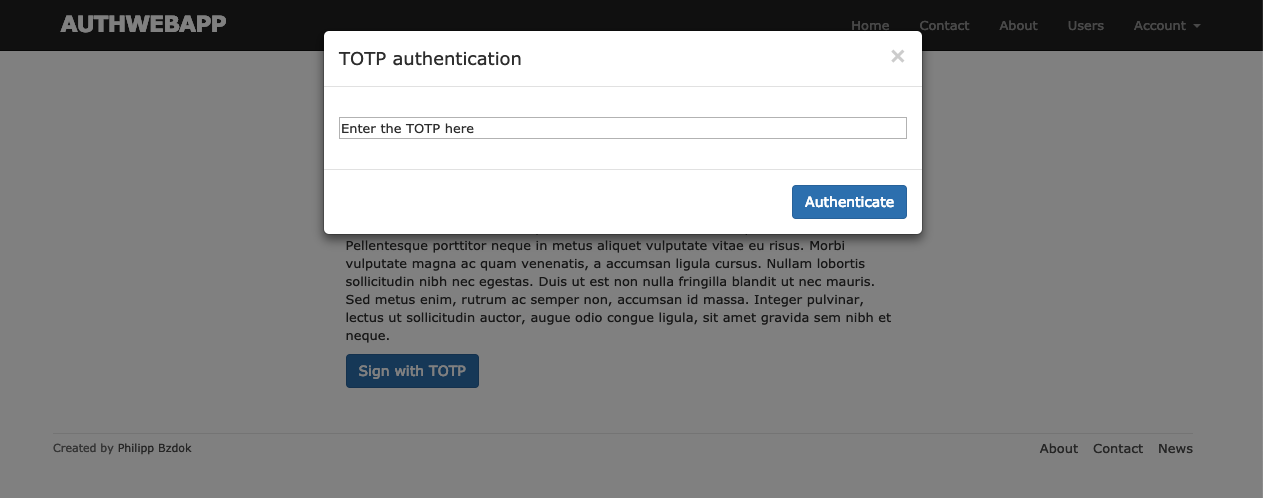
\includegraphics[width=\textwidth]{Abbildungen/Authwebapp_Signatur_via_TOTP}
    \caption{Signaturerstellung mit TOTP Authentifizierung}
    \label{fig:Authwebapp_sign_TOTP}
\end{figure}
\clearpage
\subsubsection{View}
Die \textit{Views} sind Repräsentationen der Ressourcen und können statisch sein (z.\,B. Zeilen 2-10 in Listing \ref{lst:routes.rb}) oder mithilfe von Templates und den Ressourcen dynamisch generiert werden (Zeilen 11-16 in Listing \ref{lst:routes.rb}). Die Form der \textit{View} richtet sich dabei nach der Anforderung im Request, so ist es möglich eine Ressource z.\,B. als HTML oder JSON Repräsentation anzufordern. Um die Komplexität des Prototypen gering zu halten habe ich mich jeweils auf eine Repräsentation beschränkt. Die \textit{TOTP}-Verifizierung stellt hier eine Besonderheit dar, da keine HTML Repräsentation notwendig ist. Die wichtigste \textit{View} im Kontext der \textit{TOTP}-Authentifizerung ist das Fenster welches den QR-Code abbildet. Dieses Fenster stellt eine Erweiterung zur View der Ressource User mit der URL \texttt{GET /users/:id/edit} dar, welches in Listing \ref{lst:edit.html.erb} dargestellt wird. Hier ist deutlich zu sehen wie Ruby on Rails die Infusion von Ruby Code in den Templates ermöglicht um dynamischen Inhalt zu generieren. Zeile 31 des Listings \ref{lst:edit.html.erb} zeigt die Erweiterung der View, die im Falle der aktivierten Checkbox \texttt{f.check\_box :totp\_activated} den QR-Code anzeigt. Hierbei handelt es sich um ein \texttt{Modal} aus \textit{Bootstrap} und ist Listing \ref{lst:otp_modal.html.erb} beziehungsweise Abbildung \ref{fig:Authwebapp_qr} dargestellt. Ebenfalls wird eine Javascript Datei inkludiert, welche für den asynchronen \textit{AJAX} Aufruf mit Hilfe von \textit{jQuery} an das Back-End zuständig ist. Dieses Vorgehen wurde gewählt, damit eine erfolgreiche Initialisierung des \textit{TOTP} erfolgen kann. Dazu muss der Benutzer den ihm präsentierten QR-Code mit dem \textit{Google Authenticator} scannen und anschließend das \textit{TOTP} im Fenster eingeben. Nur wenn die Verifikation durch den Server erfolgreich war kann das Authentifizierungsverfahren persistent aktiviert werden. Listing \ref{lst:otp.js} stellt die Javascript Funktionalität im Detail dar und zeigt wie die Antwort des Controllers aus Listing \ref{lst:user-controller.rb-verify-otp} interpretiert und anschließend dem Benutzer präsentiert wird. Dazu wird die \texttt{success} Callback Funktion des \textit{AJAX} Aufrufes genutzt um bei einem erfolgreichen Request die Antwort der Verifikation zu verarbeiten.

Weitere \textit{Views} der Anwendung dienen dazu dem Benutzer eine Interaktion zur ermöglichen und Daten anzuzeigen. So werden beispielsweise auf der Startseite die Nachrichten und die dazugehöhrigen Signaturen angezeigt.
\begin{listing}[htpb]
    \begin{minted}{html}
        <% provide(:title, "Edit user") %>
        <h1>Settings</h1>

        <div class="row">
            <div class="col-md-6 col-md-offset-3">
                <%= form_for(@user) do |f| %>
                <%= render 'shared/error_messages', object: f.object %>

                <%= f.label :name %>
                <%= f.text_field :name, class: 'form-control' %>

                <%= f.label :email %>
                <%= f.email_field :email, class: 'form-control' %>

                <%= f.label :password %>
                <%= f.password_field :password, class: 'form-control' %>

                <%= f.label :password_confirmation, "Confirmation" %>
                <%= f.password_field :password_confirmation, class: 'form-control' %>

                <%= f.label :totp_activated, class: "checkbox inline" do %>
                    <%= f.check_box :totp_activated %>
                    <span>TOTP activated</span>
                <% end %>

                <%= f.submit "Save changes", class: "btn btn-primary" %>
                <% end %>
            </div>
        </div>

        <%= render 'layouts/otp_modal' %>
        <%= javascript_include_tag "otp"  %>
    \end{minted}
    \caption{\texttt{edit.html.erb} - User Ressourcen Template für die edit Operation}
    \label{lst:edit.html.erb}
\end{listing}
\begin{listing}[htpb]
    \begin{minted}{html}
        <div class="modal fade" id="otp_modal" tabindex="-1" role="dialog" aria-labelledby="otp_modal_label">
        <div class="modal-dialog" role="document">
            <div class="modal-content">
            <div class="modal-header">
                <button type="button" class="close" data-dismiss="modal" aria-label="Close">
                <span aria-hidden="true">&times;</span></button>
                <h4 class="modal-title" id="otp_modal_label">TOTP verification</h4>
            </div>
            <div class="modal-body">
                <div class="qr">
                <%= raw @user.create_totp.as_html %>
                <%= text_field_tag "otp", "Enter the TOTP here", maxlength: 6 %>
                </div>
            </div>
            <div class="modal-footer">
                <button type="button" id="verify_top_btn" class="btn btn-primary">Verify</button>
            </div>
            </div>
        </div>
        </div>
    \end{minted}
    \caption{\texttt{\_otp\_modal.html.erb} - Front-End zur Anzeige des QR-Codes}
    \label{lst:otp_modal.html.erb}
\end{listing}
\begin{listing}[htpb]
    \begin{minted}{js}
        // [...]
        $('#verify_top_btn').on('click', function () {
            const id = location.pathname.split("/")[2];
            let totp = document.getElementById("otp").value;
            $.ajax({
                type: "GET",
                url: `/users/${id}/verify_otp.json`,
                data: {
                    user: {
                        totp: totp
                    }
                },
                dataType: "json",
                success: function (data) {
                    if (data["totp_valid"]) {
                        $('#otp_modal').modal('hide');
                        $("#user_totp_activated").prop("checked", true);
                        alert("TOTP successfully confirmed!")
                    }
                    else {
                        document.getElementById("otp").style.borderColor = "red";
                        alert("TOTP wrong!");
                        $("#user_totp_activated").prop("checked", false);
                    }
                },
                error: function (data) {
                    console.error("Asynchronous request failed!");
                    console.log(data)
                }
            });
        });
    \end{minted}
    \caption{\texttt{otp.js} - Javascript zur asynchronen TOTP Verifikation}
    \label{lst:otp.js}
\end{listing}
\clearpage

\section{Universal Second Factor (U2F)}
Der \textit{Universal Second Factor}, im Folgenden nur noch \textit{U2F}, ist ein offenere Standard für allgemein anwendbare Zwei-Faktor Authentifizierung. \textit{U2F} wurde von der \textit{FIDO Alliance} im Jahre 2014 spezifiziert \cite{u2fv1}. Das Verfahren basiert auf einer Challange-Response Authentifizierung und legt besonderen Wert auf die Privatsphäre des Benutzers. Der Schutz der Privatsphäre wird durch die Generierung eines neuen Schlüsselpaars pro Anwendung realisiert, sodass ein Vergleich der öffentlichen Schlüssel von mehreren Anwendungen keinen Aufschluss über das registrierte Gerät oder dessen Benutzer preisgibt. Ein Benutzer kann also ein \textit{U2F} kompatibles Gerät anwendungsübergreifend zur Authentifizierung nutzen. Außerdem ermöglicht der \textit{U2F} Standard eine Betriebssystem und Browserübergreifende Authentifizierung im Internet durch eine Javascript API und native API's für Smartphone Betriebsysteme \cite{u2fSpec}. Die Anwendung welche \textit{U2F} implementiert kann den Benutzer jederzeit zur Authentifizierung auffordern. Üblicherweise wird ein erste Faktor in Form von Benutzername und Passwort realisiert und anschließend durch eine \textit{U2F} Authentifizierung als zweiter Faktor verstärkt. \textit{U2F} Gerät können sich in diversen Formen manifestieren, beispielsweise USB-Geräte, NFC-Geräte, Bluetooth-Geräte oder bestehende Kryptographiesysteme. Eine weit verbreitete Implementierung ist ein USB-Gerät entwickelt von \textit{Yubico}, der \textit{Yubikey}\footnote{https://www.yubico.com/products/yubikey-5-overview/}. Dabei handelt es sich um eine Hardwareimplementierung in Form eines USB-Sicherheitsschlüssels mit kryptographischen Funktionen. Dieses Gerät ist zusätzlich gegen Zugriff auf die sicherheitskritischen Komponenten (Secure Element) abgesichert. Der Standard setzt sich als Ziel eine sichere ``Out-of-the-Box'' Authentifizierung zu ermöglichen indem keine weiteren Treiber benötigt werden und das Gerät über Betriebsystem APIs direkt mit dem Browser kommunizieren kann \cite{u2fSpec}. Des weiteren existieren Implementierungen des Standards welche den Zugriff auf das \textit{U2F} Gerät durch Biometrie ergänzen und somit die Bindung an den Benutzer wesentlich verstärken \cite{eyelock}.

Im Folgenden werde ich die \textit{U2F} Authentifizierung hauptsächlich am Beispiel des \textit{Yubikeys} erklären.
\subsection{Funktionsweise}
Die Authentifizierung mit einem \textit{U2F} Gerät erfordert im ersten Schritt eine Registrierung des Geräts durch den Benutzer beim Serviceprovider. Dazu muss der Benutzer das Gerät anschließen und bei Aufforderung durch eine Berührung aktivieren, wobei das Gerät ein anwendungsspezifisches kryptographisches Schlüsselpaar erstellt. Daraufhin wird dem Server ein Keyhandle und der öffentliche Schlüssel mitgeteilt und vom Server in Beziehung zum Benutzer gespeichert \cite{u2fv1}. Die Authentifizierung via \textit{U2F} ist nun für den Benutzer aktiviert und kann verwendet werden. Dazu authentifiziert sich der Benutzer in Regel erst mit dem ersten Faktor (meist Passwort) und wird dann zur \textit{U2F} Authentifizierung weitergeleitet. Die \textit{U2F} Authentifizierung erfolgt durch ein Challange-Response Protokoll indem der Server eine Challange generiert und an den Client sendet. Die Challange wird vom Client (Browser) an das \textit{U2F} Gerät weitergeleitet woraufhin der Benutzer das Gerät durch Berührung aktivieren muss. Durch die Aktivierung des Benutzers wird die Challange mithilfe des privaten Schlüssels signiert und an den Server zurück gesendet. Die Signatur kann infolge dessen vom Server mit Hilfe des öffentlichen Schlüssels verifiziert und der Benutzer authentifiziert werden. Abbildung \ref{fig:U2F-Auth} \cite{u2fTech} zeigt den schematischen Ablauf der \textit{U2F} Authentifizierung und weitere wichtige Parameter wie \texttt{origin}, \texttt{app\_id}, \texttt{channel\_id} und \texttt{counter}. Diese erweiterten Parameter dienen der Unterbindung diverser Angriffsszenarien. So wird die URI (\texttt{origin}) und die TLS Channel ID (\texttt{channel\_id}) eingesetzt um vor Phishing und Man-in-the-Middle Angriffen zu schützen. Anwendungsspezifische Authentifizierung wird durch die \texttt{app\_id} implementiert und Geräte-Klonen kann durch den \texttt{counter} unterbunden werden\footnote{Das Klonen von \textit{U2F} Geräten ist in erster Linie bei Softwarelösungen die kein Secure Element verwenden kritisch}. Zusätzlich kann die Vertrauenswürdigkeit des \textit{U2F} Geräts seitens Serviceprovider sichgestellt werden, indem im Gerät ein herstellerspezifischer Schlüssel gespeichert ist und die Antwort des Geräts damit signiert wird. Der Serviceprovider kann infolge dessen durch den allgemein bekannten öffentlichen Schlüssel des Herstellers die Authentizität des Gerätes prüfen.

\begin{figure}[htbp]
    \centering
        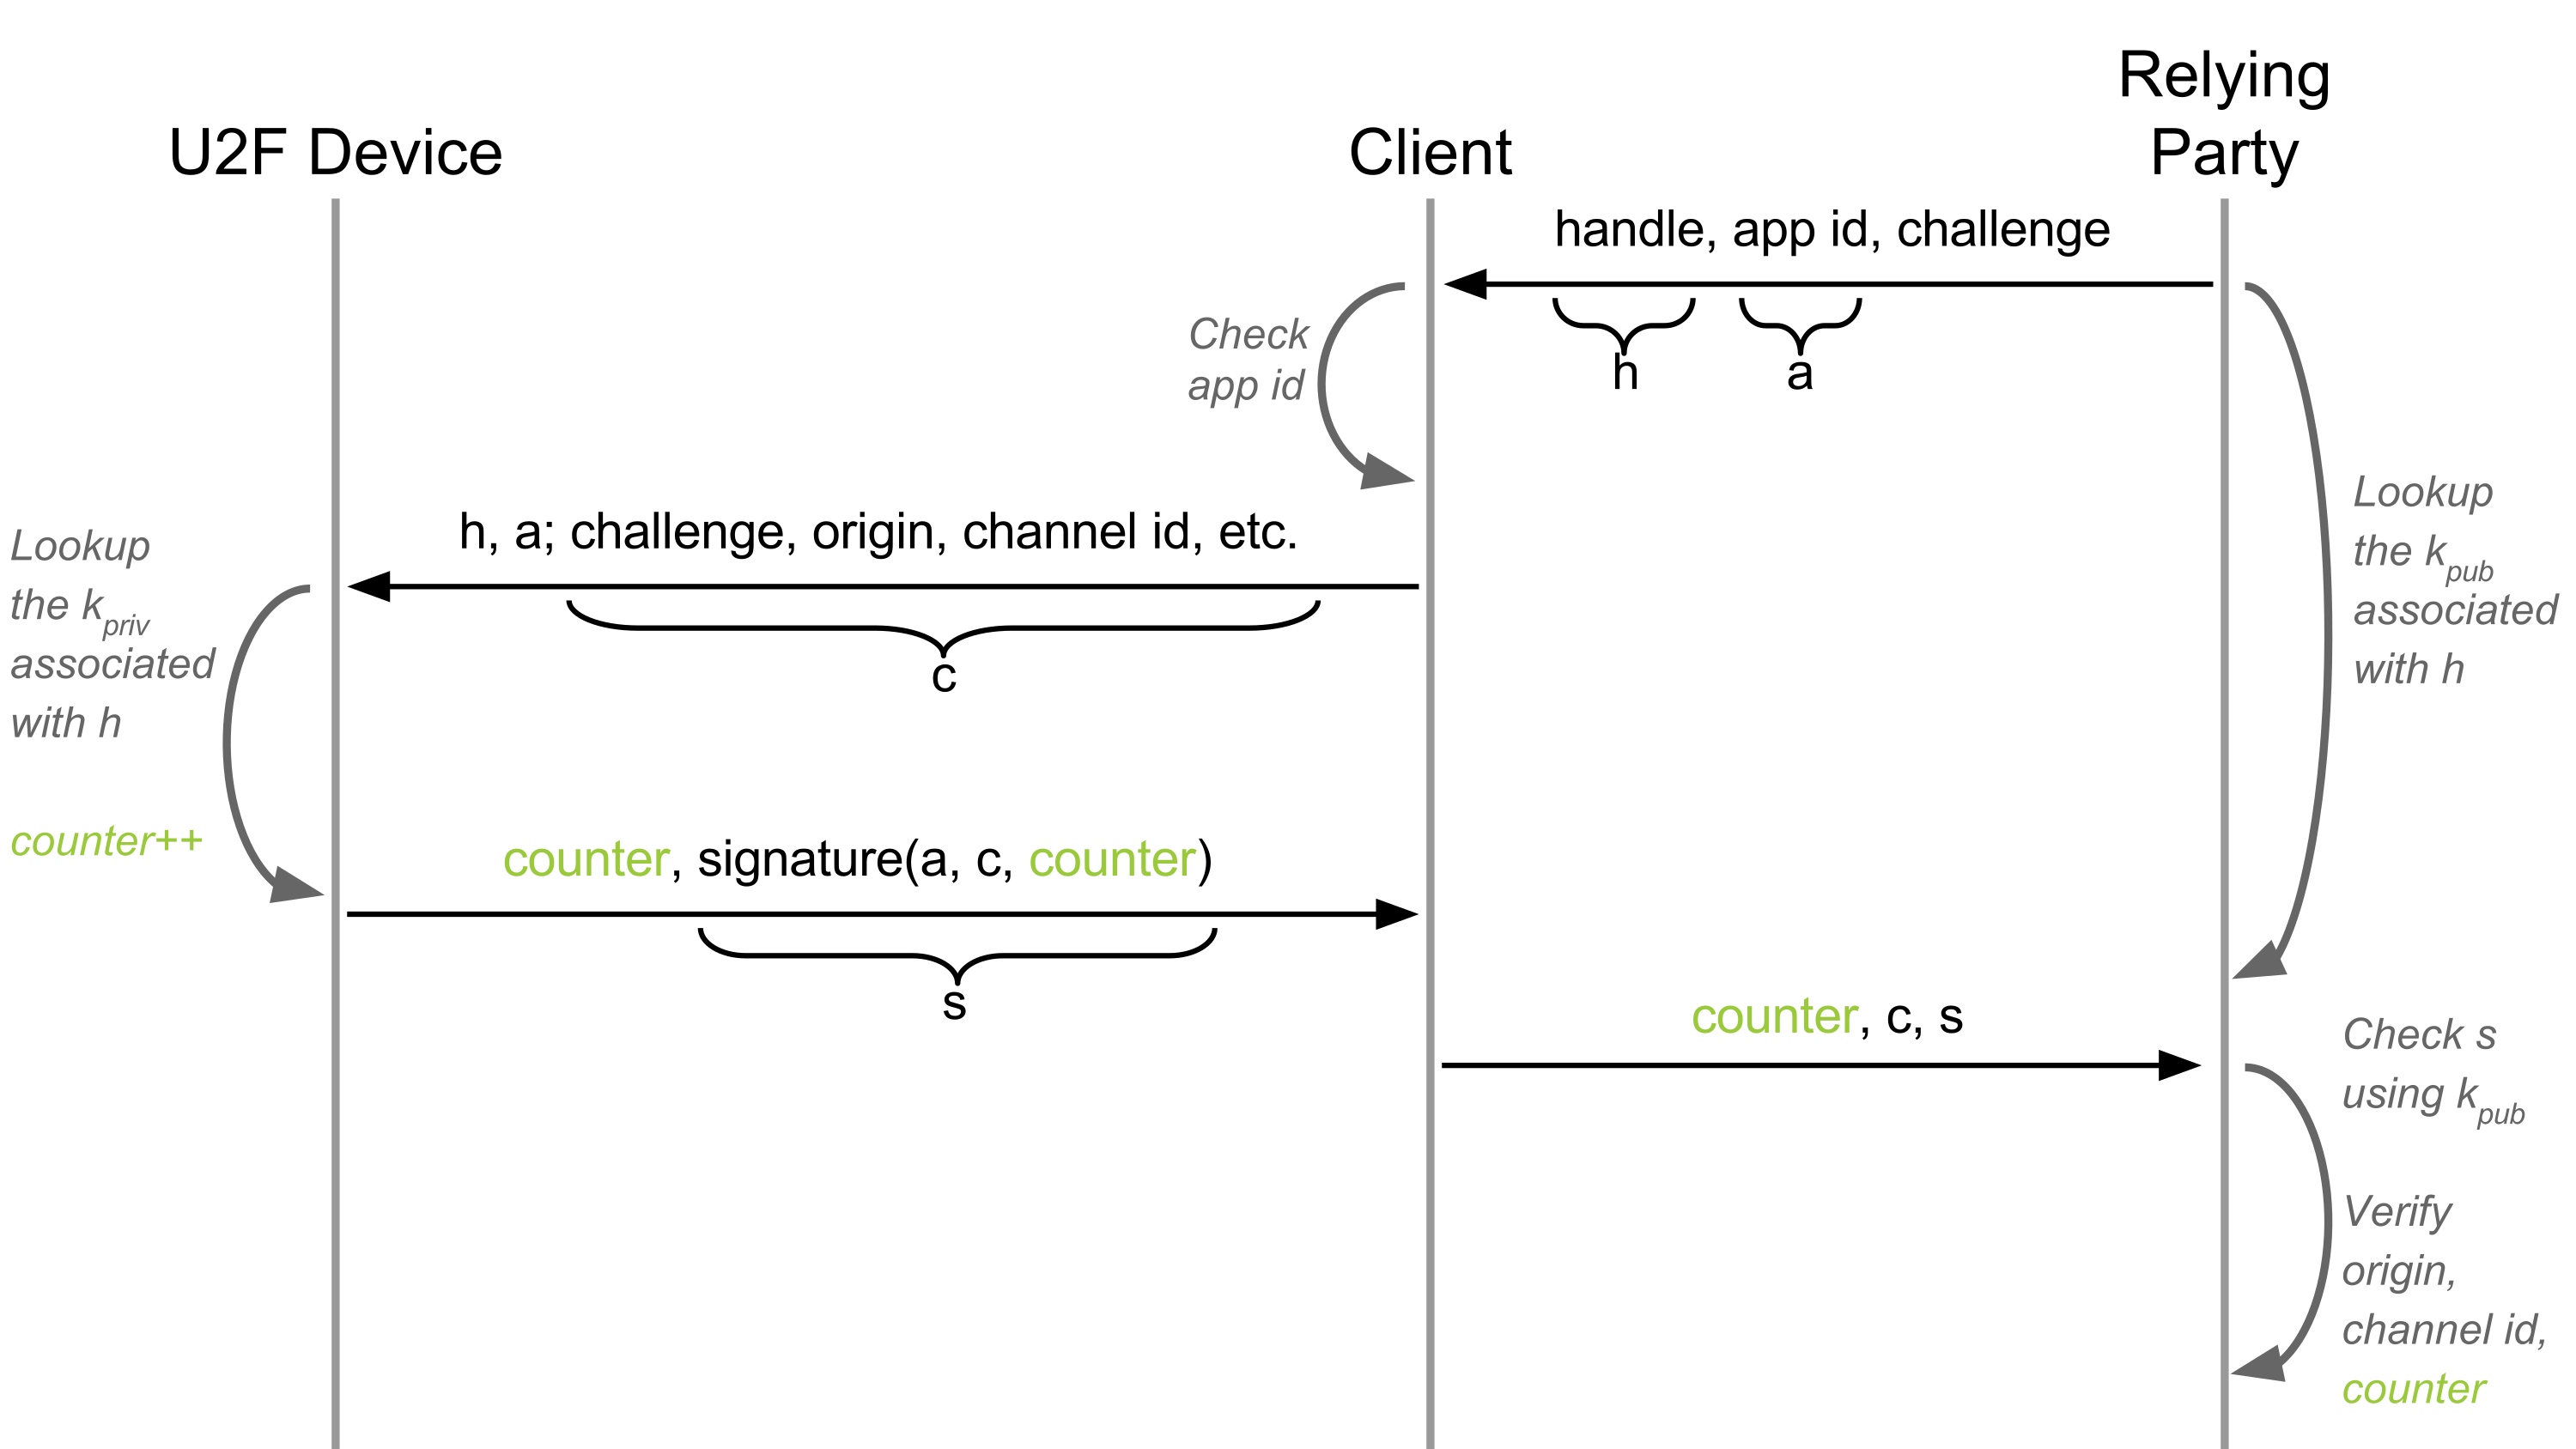
\includegraphics[width=\textwidth]{Abbildungen/yubico_u2f_flow}
    \caption{Schematischer Ablauf der U2F Authentifizierung \cite{u2fTech}}
    \label{fig:U2F-Auth}
\end{figure}
\subsection{Eigenschaften}
Die \textit{U2F} Authentifizierung nutzt ein Public-Key Kryptosystem mit nativem Browser Support (Google Chrome) um eine starke Zwei-Faktor Authentifizierung umzusetzen. Außerdem werden mittlerweile durch spezielle APIs Browser wie Firefox oder gar native mobile NFC Schnittstellen unterstützt. Durch den \textit{U2F} Standard der \textit{FIDO Alliance} mit über 170 Mitgliedern wird, ähnlich wie bei TOTP mit RFC 6238, eine hohe Interoperabilität gewährleistet. Ein wesentliches Merkmal der \textit{U2F} Authentifizierung ist die Benutzerfreundlichkeit, da der Benutzer nur durch eine einfach Interaktion mit dem Gerät einer Authentifizierung zustimmen muss und für die Verwendung von \textit{U2F} keine Installationen oder dritte Anwendungen notwendig sind. Ebenfalls von Vorteil für den Benutzer ist die anwendungsspezifische Authentifizierung, sodass ein hoher Grad an Privatsphäre möglich ist. Die \textit{U2F} Authentifizierung verhindert durch die Verwendung der öffentlichen Schlüssel pro Anwendung den Abbgleich von benutzerbezogenen Authentifizierungsdaten zwischen Serviceprovidern und somit die Rückverfolgung des Benutzers. Auch das Gerät selbst weist keine nach Außen hin eindeutige Gerätekennung auf. Da \textit{U2F} ein offener Standard ist, existieren auch Open-Source Softwarelösungen für das authentifizierungs Back-End  wodurch die Komplexität der Implementierung eines solchen Systems erheblich sinkt. Die wichtigste Eigenschaft der \textit{U2F} Authentifizierung ist die Sicherheit, welche durch die Verwendungung eines Public-Key Kryptosystems gewährleistet wird. So kann die Signatur, welche im Rahmen der Authentifizierung erstellt wird, zweifeilsfrei vom Serviceprovider verifiziert und zur Authentifizierung des Benutzers genutzt werden. In Verbindung mit einem gegen Zugriff gesicherten Secure Element in Form eines Hardware Security Keys (wie der \textit{Yubikey 5}) ergibt sich ingesamt ein sehr hohes Sicherheitsniveau.

Im Vergleich zur \textit{SMS-TAN} hat die Authentifizierung mit \textit{U2F} viele Vorteile. Insbesondere die Verwendung eines Secure Element mit einem Public-Key Kryptosystem macht eine solche Authentifizierung sehr sicher. Im Gegensatz zum verwendeten Mobiltelefon mit der unsicheren Übertragung der TAN über das Mobilfunknetzwerk geschieht die Kommunikation bei \textit{U2F} über eine verschlüsselte TLS Verbindung unter Verwendung eines Challange-Response Protokolls. Das Challange-Response Protokoll bietet gegenüber der \textit{SMS-TAN} zusätzlichen Schutz bei einem Man-in-the-Middle Angriff, da ein Angreifer durch das Abfangen der Challange keine Authentifizierung im Namen des Benutzers durchführen kann. Ebenfalls lässt sich ein Sicherheitsschlüssel (z.\,B. \textit{Yubikey}) sicherer Aufbewahren als ein Mobiltelefon, welches einen Alltagsgegenstand darstellt.
\subsection{Sicherheit}
Die Sicherheit der \textit{U2F} Authentifizierung basiert auf einem Public-Key Kryptographiesystem. Dabei werden Signaturen (vgl. Kapitel \ref{sec:signatur}) verwendet um den Benutzer eindeutig zu authentifizieren. Die Verwendung von digitalen Signaturen in Verbindung mit einem Challange-Response Protokoll und sicheren Hardware-Speichern (Secure Element) ermöglichen ein sehr hohes Sicherheitsniveau. Die \textit{U2F} Authentifizierung macht sich die Eigenschaften der digitalen Signatur zur nutze um eine sichere Authentifizierung zu gewährleisten. Inbesondere \emph{Authentizität}, \emph{Fälschungssicherheit}, \emph{nicht-Wiederverwertbarkeit} und \emph{Unveränderbarkeit} sind Eigenschaften der Signatur die von großem Vorteil bei einer Authentifizierung sind. Hardwaregestützte Implementierungen des \textit{U2F} Standards, wie der \textit{Yubikey}, repräsentieren die Authentifizierung durch Besitztum besonders gut, da ein solcher Sicherheitsschlüssel einmalig ist, nicht vervielfältigt werden kann und dem Benutzer physisch vorliegen muss. Eine Besonderheit von \textit{U2F} ist die Sicherheit vor Datenleaks beim Serviceprovider. Im Falle eines Hackingangriffs auf die Datenbank eines Serviceproviders ist es nicht möglich anhand des dort hinterlegten öffentlichen Schlüssels das Gerät, welches zur Authentifizierung genutzt wurde, ausfindig zu machen oder die so gewonnenen Daten zur Authentifizierung bei einem anderen Dienst zu nutzen. Das stellt im Gegensatz zu Passwörtern, welche oft auf mehreren Plattformen wiederverwendet werden, einen großen Vorteil dar. Auch verglichen mit der \textit{SMS-TAN} ist das ein eindeutiger Vorteil, da in einem solchen Angriffsszenario die Handynummer des Benutzers offengelegt werden könnte.
\subsection{Schwächen}
Schwächen weißt das \textit{U2F} Verfahren inbesondere bei unsachgemäßer Handhabung des Sicherheitsschlüssels oder falscher Implementierung auf. Es steht in der Verantwortung der Benutzers das \textit{U2F} Gerät sicher zu verwahren und vor unbefugtem Zugriff zu schützen da, am Beispiel des Yubikeys, meist nur eine einfache Interaktion mit dem Gerät reicht um eine Authentifizerung durchzuführen. Abhilfe dagegen schaffen Implementierungen wie \textit{Myris}\footnote{https://www.eyelock.com/index.php/access-control/myris}, welche zusätzliche biometrische Merkmale wie die Iris erfordern. Deshalb ist eine Authentifizierung mit \textit{U2F} immer in Verbindung mit einem weiteren Faktor zu empfehlen. Ein weiteres Risko ist der Verlust der Hardware, wodurch der Benutzer den Zugriff auf sein Benutzerkonto verliehrt falls er keine Backup-Authentifizierung eingerichtet oder eine zweites \textit{U2F} Gerät zuvor registriert hat. Neben den benutzerspezifischen Risikofaktoren existieren ebenfalls technische Anforderungen um eine sichere Authentifizierung zu ermöglichen. So ist die Verwendung von verschlüsselten Übertragungskanälen zwangsweise erforderlich. Die \textit{FIDO Alliance} weist in der \textit{Universal 2nd Factor (U2F) Overview} \cite{u2fSpec} darauf hin das eine Schwachstelle die Interaktion des Gerätes mit Malware ist, solange der Zugriff über Anwendungen geschieht welche im \textit{User Space} agieren. Das \textit{U2F} Gerät kann einen ``guten'' Client nicht von einem ``bösen'' unterscheiden, sodass es prinzipiell möglich ist eine Registrierung bei einem bösartigen Serviceprovider (\texttt{origin}) durchzuführen. Verhindert werden soll dies durch direkten Zugriff auf das Gerät durch das Betriebssystem, jedoch existieren solche APIs gegenwärtig noch nicht.
\subsection{Implementierung}
In diesem Kapitel möchte ich eine prototypische \textit{U2F} Authentifizierung auf Basis einen \textit{Ruby on Rails} Webanwendung darstellen. Die Webanwendung ermöglicht es dem Benutzer sich zu registrieren und mit Hilfe der Zwei-Faktor Authentifizierung eine Nachricht zu signieren. Die Implementierung basiert auf der Anwendung aus Kapitel \ref{sec:TOTP} und erweitert diese. Aus diesem Grund ergeben sich einige Parallelen in gemeinsamen Komponenten wie dem \textit{User} und \textit{Message Model}, der Aktivierung des Benutzerkontos über eine E-Mail und der Aktivierung der Multi-Faktor Authentifizierung. Die Aktivierung der \textit{U2F} Authentifizierung setzt das angeschlossene Gerät, die Benutzerinteraktion mit dem Gerät und einen erfolgreichen Registrierungsprozess im Back-End voraus. Abbildung \ref{fig:Authwebapp_u2f_init} zeigt schematisch den \textit{U2F} Registrierungsprozess in der Webanwendung analog zu Abbildung \ref{fig:totp-init}. Die Authentifizierung mit \textit{U2F} erfolgt ebenfalls ähnlich wie mit TOTP, jedoch wird der Benutzer ausschließlich zur Interaktion mit dem Gerät aufgefordert und muss keine Eingabe tätigen (siehe Abb. \ref{fig:Authwebapp_u2f_auth}). Die Aufforderung an den Benutzer wird ihm visuell im Browser mitgeteilt, wobei der aktive \textit{Yubikey} anfängt zu blinken um seine Bereitschaft zu signalisieren. Dieser halbautomatisierte Ablauf wird durch die \textit{U2F} Javascript API\footnote{https://github.com/fido-alliance/google-u2f-ref-code/blob/master/u2f-gae-demo/war/js/u2f-api.js} ermöglicht. Meine Implementierung nutzt die Javascript API um, nach einer erfolgreichen Authentifizerung durch \texttt{u2f.sign}, automatisch die Signaturerstellung anzustoßen (Details dazu im View Kapitel). Wie im Kapitel \ref{sec:TOTPImpl} werde ich die Implementierung innerhalb der Komponenten des MVC-Frameworks beschreiben um eine gute Gegenüberstellung zu ermöglichen. Für die Authentifizierung mit \textit{U2F} ist ein kompatibler Browser und ein kompatibles Gerät notwendig. Der Browser welcher zum testen der Anwednung benutzt wurde ist \textit{Google Chrome 72.0} und das \textit{U2F} Gerät ist der \textit{Yubikey 5} von \textit{Yubico}.
\begin{figure}[htbp]
    \centering
        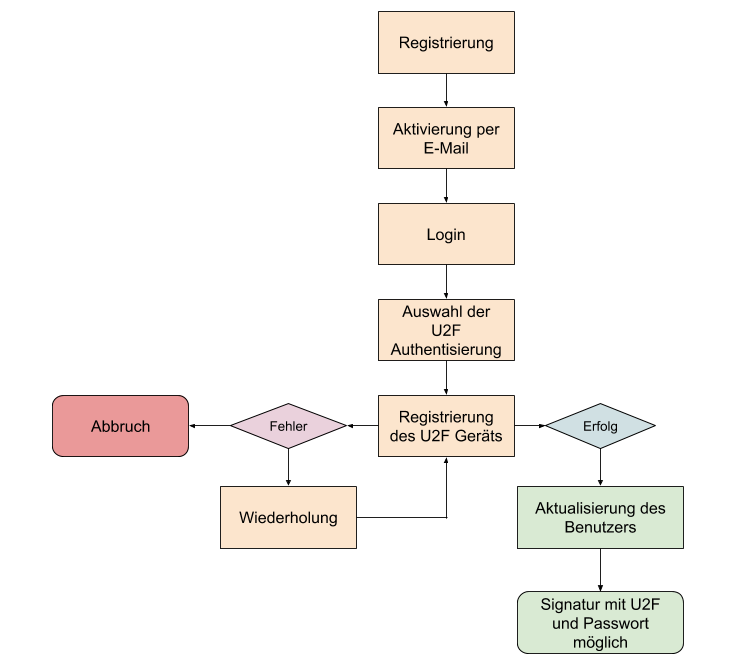
\includegraphics[width=\textwidth]{Abbildungen/Ablauf_U2F_Initialisierung}
    \caption{Schematischer Ablauf der U2F Initialisierung in der Webanwendung}
    \label{fig:Authwebapp_u2f_init}
\end{figure}
\begin{figure}[htbp]
    \centering
        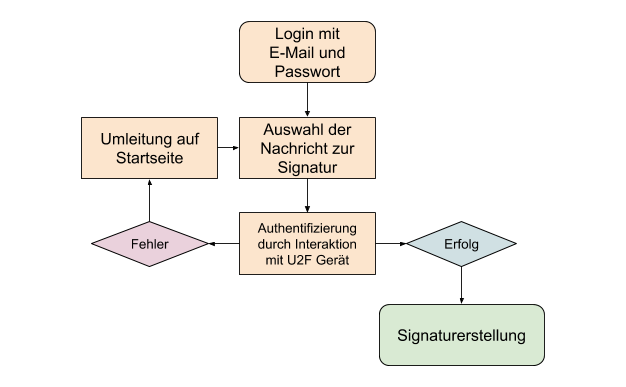
\includegraphics[width=\textwidth]{Abbildungen/Ablauf_U2F}
    \caption{Schematischer Ablauf der U2F Authentifizierung in der Webanwendung}
    \label{fig:Authwebapp_u2f_auth}
\end{figure}
\clearpage
\subsubsection{Model}
Das \textit{User Model} wurde im Vergleich zu Kapitel \ref{sec:TOTPImpl} erweitert um die Registrierung eines oder mehrerer \textit{U2F} Geräte zu ermöglichen. Nicht verändert haben sich die Validitätsprüfungen der übergreifenden Parameter wie Name, E-Mail und Passwort. Programatisch wurde das \textit{User Model} in Beziehung mit dem neuen \textit{U2F Registration Model} gesetzt, wie in Listings \ref{lst:user.rb-u2f_Relationship} und \ref{lst:u2f_registration.rb} zu sehen. Um eine aktive \textit{U2F} Authentisierung pro Benutzer zu speichern wurde das boolsche Datenbankfeld \texttt{u2f\_activated} der User Tabelle aus Tabelle \ref{table:db-user} hinzugefügt. Gänzlich neu ist die Datenbanktabelle der \textit{U2F} Registrierungen, welche in Tabelle \ref{table:db-u2f} dargestellt ist. Die erfolgreiche Registrierung eines \textit{U2F} Geräts erstellt folglich einen Datenbankeintrag in Beziehung zum aktuell angemeldeten Benutzer. Dieser Datenbankeintrag kann zu einem späteren Zeitpunkt zur Authentifizerung des Benutzers herangezogen werden. Dazu wird anhand des \texttt{key\_handle} aus dem Request der entsprechende Eintrag gesucht und die Signatur durch den zugehörigen öffentlichen Schlüssel validiert. Weitere Anpassungen an den Models (z.\,B. \textit{Message Model}) mussten für die \textit{U2F} Authentifizerung nicht implementiert werden. 
\begin{listing}[htpb]
    \begin{minted}{ruby}
        class User < ApplicationRecord
            has_many :messages, dependent: :destroy
            has_many :u2f_registrations, dependent: :destroy
            has_secure_password
        # [...]
    \end{minted}
    \caption{\texttt{User.rb} - Beziehung zu U2F Registrierung}
    \label{lst:user.rb-u2f_Relationship}
\end{listing}
\begin{listing}[htpb]
    \begin{minted}{ruby}
        class U2fRegistration < ApplicationRecord
            belongs_to :user
        end
    \end{minted}
    \caption{\texttt{u2f\_registration.rb} - U2F Registrierungsmodel}
    \label{lst:u2f_registration.rb}
\end{listing}
\begin{table}[htbp]
    \begin{tabularx}{\textwidth}{ lX }
        \toprule
        Spalte & Beschreibung \\ 
        \midrule
        \texttt{certificate} & Zertifikat welches bei der Aktivierung des Gerätes generiert wurde \\
        \texttt{key\_handle} & String als Referenz auf den verwendeten Schlüssel \\
        \texttt{public\_key} & Öffentlicher Schlüssel der zur Authentifizerung des Benutzers dient \\
        \texttt{counter} & Anzahl der Verwendungung \\
        \texttt{user\_id} & ID des in Beziehung stehenden Benutzers \\
        \texttt{created\_at} & Erstellungsdatum der Registrierung \\
        \texttt{updated\_at} & Aktualisierungsdatum \\
        \bottomrule
    \end{tabularx}
    \caption{Datenbanktabelle - U2F Registrierung}
    \label{table:db-u2f}
\end{table}
\clearpage
\subsubsection{Controller und Routen}
Im Gegensatz zu den Models mussten umfangreiche Ergänzungen an den \textit{Controller} und \textit{Routen} vorgenommen werden. Die \textit{U2F} Registrierung erfolgt über eine neue URL (siehe Listing \ref{lst:routes.rb-u2f}), welche die Operation \texttt{create} des \textit{U2F Registrations Controller} aufruft. Ausgelöst wird dieser Aufruf durch die Registrierung der Benutzerinteraktion mit dem Gerät durch die Javascript API. Ziel der \texttt{create} Funktion ist die Validierung der vom Client beziehungsweise \textit{U2F} Gerät übermittelten Daten und die anschließende Speicherung in der Datenbank. Diese Operation geschieht immer im Kontext des angemeldeten Benutzers um eine konsistente Beziehung der Models herzustellen. Listing \ref{lst:u2f_registrations_controller.rb} zeigt die Funktion zur Verarbeitung eines POST Requests, welcher durch die Javascript API an die URL \texttt{/u2f\_registration} gesendet wurde. Für die \textit{U2F} Registrierung und Authentifizerung wurde die Ruby Bibiliothek \textit{ruby-u2f}\footnote{https://github.com/castle/ruby-u2f} verwendet. Meine Implementierung der Registrierung und der Authentifizerung hier stützt sich stark auf die Beispielimplementierung der Bibliothek. Mit den vom Gerät stammenden Parametern des POST Requests wird mit Hilfe der \textit{ruby-u2f} Bibliothek ein \texttt{response} Objekt erzeugt und wiederrum als Parameter an die \ruby{u2f.register!} Funktion (Siehe Zeile 7 aus Listing \ref{lst:u2f_registrations_controller.rb}) übergeben. Falls hierbei keine Fehler auftreten, können die für die Datenbank relevanten Daten aus dem \texttt{registration} Objekt extrahiert und in der Datenbank als \textit{U2F} Registrierung gespeichert werden.

Die Authentifizierung mit \textit{U2F} ist ebenfalls in einem seperaten Controller implementiert und erfodert kein zugehöriges Model, da keine persistenten Daten gespeichert werden müssen. In Listing \ref{lst:routes.rb-u2f} ist zu erkennen, dass die URL \texttt{/u2f\_authentication} die \texttt{create} Funktion des \textit{U2F Authentication Controller} aufruft. Eine Authentifizerung wird analog zur Registrierung durch einen POST Request mit JSON Inhalt durch die Javascript API ausgelöst. Listing \ref{lst:u2f_authentications_controller.rb} zeigt wie aus dem JSON Objekt mit Hilfe der \textit{ruby-u2f} Bibliothek ein \texttt{response} Objekt erzeugt wird. Bestandteil dieses Objektes ist das \texttt{key\_handle}, welches zum laden eines \textit{U2F} Registrierungs Eintrags der Datenbank verwendet wird. Falls ein solches \texttt{key\_handle} noch nicht hinterlegt ist, wird der Benutzer aufgefordert zuerst ein \textit{U2F} Gerät zu registrieren. Zusammen mit der Challange, welche vor der Signaturerstellung generiert wurde (siehe Listing \ref{lst:message_controller.rb-u2f}), und der \texttt{response} als Parameter wird die \ruby{u2f.authenticate!} Funktion aufgerufen. Die von \textit{ruby-u2f} generierte Challange ist ein 32 Byte langer zufälliger String. Die Challnge wird genutzt um die vom Gerät erstellte Signatur im Rahmen der \ruby{u2f.authenticate!} Funktion zu validieren. Falls diese Funktion erfolgreich ausgeführt wurde, wird die Challange gelöscht, der Counter inkrementiert und die Nachricht mit Hilfe des privaten Schlüssels des Benutzers signiert.

\begin{listing}[htpb]
    \begin{minted}{ruby}
        # [...]
        post '/u2f_registration', to: 'u2f_registrations#create'
        post '/u2f_authentication', to: 'u2f_authentications#create'
        # [...]
    \end{minted}
    \caption{\texttt{routes.rb} - Definition der für \textit{U2F} notwendigen Routen}
    \label{lst:routes.rb-u2f}
\end{listing}
\begin{listing}[htpb]
    \begin{minted}{ruby}
        class U2fRegistrationsController < ApplicationController
            skip_before_action :verify_authenticity_token

            def create
                response = U2F::RegisterResponse.load_from_json(params[:response])
                registration = begin
                    u2f.register!(session[:challenges], response)
                rescue U2F::Error => e
                    return "Unable to register: <%= e.class.name %>"
                ensure
                    session.delete(:challenges)
                end

                @u2f_registration = current_user.u2f_registrations.build(certificate:         registration.certificate, key_handle: registration.key_handle, public_key: registration.public_key, counter: registration.counter)                                                                                          
                @u2f_registration.save
            end
        end
    \end{minted}
    \caption{\texttt{u2f\_registrations\_controller.rb} - \textit{U2F} Registrierungsoperation}
    \label{lst:u2f_registrations_controller.rb}
\end{listing}
\begin{listing}[htpb]
    \begin{minted}{ruby}
        class U2fAuthenticationsController < ApplicationController
            skip_before_action :verify_authenticity_token

            def create
                response = U2F::SignResponse.load_from_json(params[:response])

                registration = U2fRegistration.find_by_key_handle(response.key_handle)
                return 'Need to register first' unless registration

                begin
                    u2f.authenticate!(session[:challenge],
                                        response,
                                        Base64.decode64(registration.public_key),
                                        registration.counter)
                rescue U2F::Error => e
                    return "Unable to authenticate: <%= e.class.name %>"
                ensure
                    session.delete(:challenge)
                end

                registration.update(counter: response.counter)
                sign_message
                redirect_to root_url
            end

            private

            def sign_message
                pkey = OpenSSL::PKey::RSA.new(current_user.private_key)
                message = Message.find(params[:message_id])
                message.sign_content(pkey)
                message.save
            end
        end
    \end{minted}
    \caption{\texttt{u2f\_authentications\_controller.rb} - \textit{U2F} Authentifizungsoperation}
    \label{lst:u2f_authentications_controller.rb}
\end{listing}
\begin{listing}[htpb]
    \begin{minted}{ruby}
        # [...]
        def initialize_u2f_authentication
            # Fetch existing Registrations from your db
            key_handles = U2fRegistration.all.map(&:key_handle)
            return 'Need to register first' if key_handles.empty?
        
            # Generate SignRequests
            @app_id = u2f.app_id
            @sign_requests = u2f.authentication_requests(key_handles)
            @challenge = u2f.challenge
        
            # Store challenge. We need it for the verification step
            session[:challenge] = @challenge
        end
        # [...]
    \end{minted}
    \caption{\texttt{message\_controller.rb} - \textit{U2F} Initialisierung}
    \label{lst:message_controller.rb-u2f}
\end{listing}
\clearpage
\subsubsection{View}
Die Implementierung der Views im Kontext der \textit{U2F} Authentifizerung ist im Vergleich zu TOTP  komplexer, da diese die Javascript Funktionalität zur Kommunikation mit dem Gerät enthalten. Um die Benutzerinteraktion so einheitlich wie möglich zu halten, wird die \textit{U2F} Registration, wie bei TOTP in einem Bootstrap \textit{Modal} abgewickelt und benötigt deshalb keine eigene gerenderte View. Die View die das \textit{Modal} beinhaltet wird, wie bei TOTP, von \texttt{/users/:id/edit} bereitgestellt und repräsentiert den angemeldeten Benutzer. Im Gegensatz zu TOTP erfordert die Registrierung und Authentifizerung mit \textit{U2F} keine Eingabe vom Benutzer. Stattdessen wird der Benutzer durch das \textit{Modal} zur Interaktion mit dem Gerät aufgefordert, wie in Abbildung \ref{fig:Authwebapp_u2f_reg} zu sehen ist. Während diesem Prozess blinkt das Gerät um Bereitschaft zur Interaktion zu signalisieren. Durch die Benutzerinteraktion wird der Registrierungsprozess ausgelöst, indem ein POST Request an die entsprechende URL im Back-End gesendet wird. Listing \ref{lst:u2f_modal.html.erb} zeigt die Verwendung des \textit{Modal} in Kombination mit der \textit{U2F} Javascript API und den vom Back-End bereitgestellten Parametern \texttt{appId}, \texttt{registerRequests} und \texttt{signRequests}. Um die Funktionalität des Skripts zu gewährleisten, muss die Javascript API\footnote{https://github.com/fido-alliance/google-u2f-ref-code/blob/master/u2f-gae-demo/war/js/u2f-api.js} in der Asset-Pipeline von Ruby on Rails aufgenommen werden. Die Benutzerinteraktion führt zum Senden der \texttt{hidden\_u2f\_form} durch die Delegation an die \texttt{u2f.register} Funktion, welche die Schnittstelle zur API darstellt. Nach der Verarbeitung im Back-End durch den \textit{U2F Registration Contoller}, wird der Benutzer durch einen Alert auf den erfolgreichen Abschluss des Prozesses hingewiesen. Infolge dessen verschwindet das \textit{Modal}, die entsprechende Checkbox bleibt aktiv und der Benutzer kann durch eine finale Bestätigung die Änderungen persistent speichern lassen.
\begin{figure}[htbp]
    \centering
        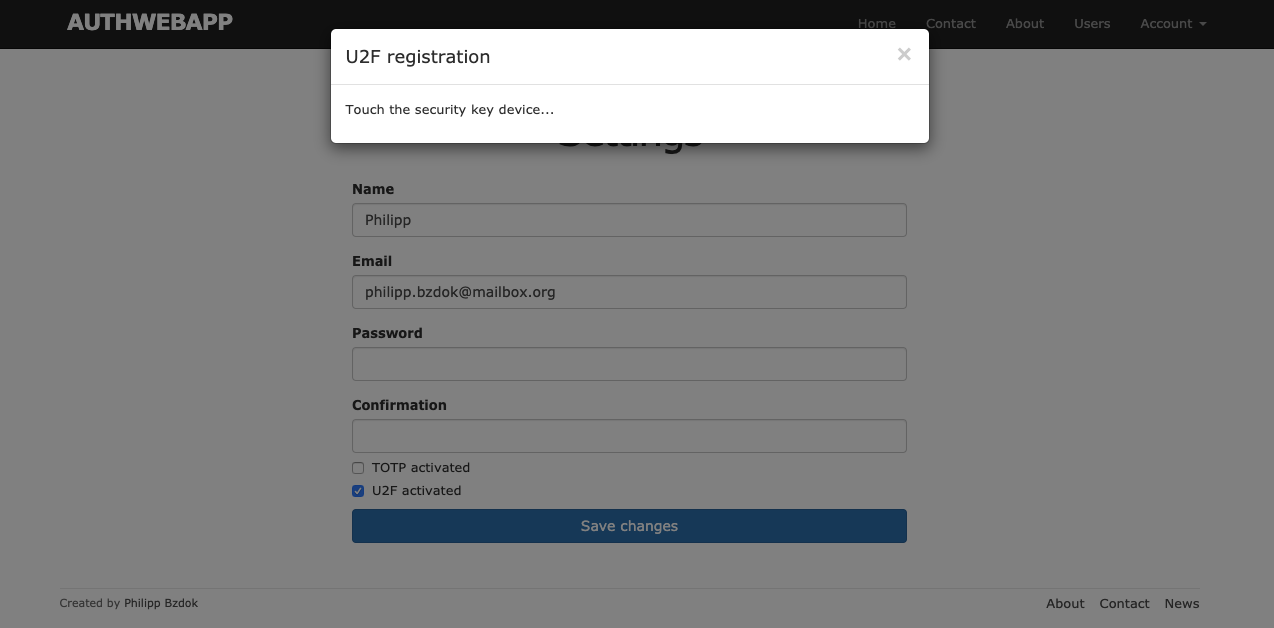
\includegraphics[width=\textwidth]{Abbildungen/Authwebapp_U2F_Registrierung}
    \caption{Aufforderung des Benutzers zur Interaktion mit dem \textit{U2F} Gerät}
    \label{fig:Authwebapp_u2f_reg}
\end{figure}
Möchte der Benutzer eine Nachricht signieren und hat wie oben beschrieben die Registrierung abgeschlossen, kann er dies durch die Authentifizerung mit \textit{U2F} tun. Analog zur Signatur mit TOTP wählt der Benutzer die Nachricht aus und wird auf die View zur Bearbeitung der Nachricht weitergeleitet (\texttt{messages/:id/edit}). Abhängig vom aktivierten Authentifizierungsverfahren (hier \textit{U2F}) kann der Benutzer durch Drücken des entsprechenden Buttons die Authentifizierung starten. Wie bei der Registrierung wird dem Benutzer ein \textit{Modal} präsentiert, welches ihn zur Interaktion mit dem bereits blinkenden Gerät auffordert. Listing \ref{lst:u2f_auth_modal.html.erb} zeigt wie die Interaktion des Benutzers, ähnlich zur Registrierungen, die \texttt{hidden\_u2f\_authentication\_form} an das Back-End übermittelt. Bei der Authentifizerung wird jedoch die \texttt{u2f.sign} Funktion der Javascript \textit{U2F} API verwendet um die vom Back-End bereitgestellte \texttt{challenge} in Verbindung mit weiteren Parametern vom Gerät signieren zu lassen. Diese Signatur wird automatisch an das Back-End weitergeleitet und vom \textit{U2F Authentication Controller} verifiziert. Dieser Prozess findet im Kontext der zu signierenden Nachricht statt, sodass eine erfolgreiche Authentifizerung anhand der vom Gerät erstellten Signatur die Signatur der Nachricht auslöst. Die Nachricht wird in diesem Schritt aktualisiert und in der Datenbank gespeichert. Der erfolgreiche Abschluss des Prozesses hat zur Folge, dass der Benutzer auf die Startseite weitergeleitet wird und dort die Signatur der Nachricht inspizieren kann.
\begin{listing}[htpb]
    \begin{minted}{html}
<div class="modal fade" id="u2f_modal" tabindex="-1" role="dialog" aria-labelledby="u2f_modal_label">
  <div class="modal-dialog" role="document">
    <div class="modal-content">
      <div class="modal-header">
        <button type="button" class="close" data-dismiss="modal" aria-label="Close">
          <span aria-hidden="true">&times;</span></button>
        <h4 class="modal-title" id="u2f_modal_label">U2F registration</h4>
      </div>
      <div class="modal-body">
        <p>Touch the security key device...</p>
        <form id="hidden_u2f_form" action="/u2f_registration" method="post">
          <input type="hidden" name="response">
        </form>
      </div>
    </div>
  </div>
</div>

<script>
    let appId = <%= @app_id.to_json.html_safe %>;
    let registerRequests = <%= @registration_requests.to_json.html_safe %>;
    let signRequests = <%= @sign_requests.as_json.to_json.html_safe %>;
    u2f.register(appId, registerRequests, signRequests, function (registerResponse) {
        var form, reg;
        if (registerResponse.errorCode) {
            $('#u2f_modal').modal('hide');
            return alert("Registration error: "
                + registerResponse.errorCode
                + "\nMore at: https://developers.yubico.com/U2F/Libraries/Client_error_codes.html");
        }

        form = document.getElementById('hidden_u2f_form');
        let response = document.querySelector('[name=response]');

        response.value = JSON.stringify(registerResponse);

        form.submit();
        $('#u2f_modal').modal('hide');
        $("#user_u2f_activated").prop("checked", true);
        alert("U2F successfully initialized");
    });
</script>
    \end{minted}
    \caption{\texttt{\_u2f\_modal.html.erb} - Front-End der \textit{U2F} Registrierung}
    \label{lst:u2f_modal.html.erb}
\end{listing}

\begin{listing}[htpb]
    \begin{minted}{html}
<div class="modal fade" id="u2f_authentication_modal" tabindex="-1" role="dialog" aria-labelledby="u2f_modal_label">
  <div class="modal-dialog" role="document">
    <div class="modal-content">
      <div class="modal-header">
        <button type="button" class="close" data-dismiss="modal" aria-label="Close">
          <span aria-hidden="true">&times;</span></button>
        <h4 class="modal-title" id="u2f_modal_label">U2F authentication</h4>
      </div>
      <div class="modal-body">
        <p>Please activate the security key device...</p>
        <form action="/u2f_authentication" method="post" id="hidden_u2f_authentication_form">
          <input type="hidden" name="response">
          <input type="hidden" name="message_id" value="<%= @message.id %>">
        </form>
      </div>
    </div>
  </div>
</div>

<script>
    var signRequests = <%= @sign_requests.to_json.html_safe %>;
    var challenge = <%= @challenge.to_json.html_safe %>;
    var appId = <%= @app_id.to_json.html_safe %>;
    var message_id = location.pathname.split("/")[2];

    u2f.sign(appId, challenge, signRequests, function (signResponse) {
        var form, reg;

        if (signResponse.errorCode) {
            return alert("Authentication error: " + signResponse.errorCode);
        }

        form = document.getElementById('hidden_u2f_authentication_form');
        response = document.querySelector('[name=response]');

        response.value = JSON.stringify(signResponse);
        form.submit();
    });
</script>
    \end{minted}
    \caption{\texttt{\_u2f\_authentication\_modal.html.erb} - Front-End der \textit{U2F} Authentifizerung}
    \label{lst:u2f_auth_modal.html.erb}
\end{listing}

\chapter{Ergebnisse}

\chapter{Zusammenfassung}

% ----------------------------------------------------------------
% Quellcodeverzeichnis
% ----------------------------------------------------------------
\clearpage
\phantomsection
\addcontentsline{toc}{chapter}{Quellcodeverzeichnis}
\listoflistings
\clearpage

% ----------------------------------------------------------------
% Tabellenverzeichnis
% ----------------------------------------------------------------
\phantomsection
\addcontentsline{toc}{chapter}{Tabellenverzeichnis}
\listoftables
\clearpage

% ----------------------------------------------------------------
% Abbildungsverzeichnis
% ----------------------------------------------------------------
\phantomsection
\addcontentsline{toc}{chapter}{Abbildungsverzeichnis}
\listoffigures
\clearpage

% ----------------------------------------------------------------
% Literaturverzeichnis
% ----------------------------------------------------------------
\phantomsection
\addcontentsline{toc}{chapter}{Literaturverzeichnis}
\bibliographystyle{ieeetr}
\bibliography{Literaturverzeichnis}

\end{document}